\documentclass[notitlepage, reprint, nofootinbib]{revtex4-1}
\usepackage[utf8]{inputenc}

% Mathematics and symbols:
\usepackage{amsmath, gensymb, amsthm, physics, mhchem, amssymb}
% Algorithms: 
\usepackage{algorithm}
\usepackage{algpseudocode}
% Figures:
\usepackage{tikz, graphicx}
\usepackage[caption=false]{subfig}

% Other:
\usepackage{hyperref}


% Document formatting 
\setlength{\parskip}{1mm}
\setlength{\parindent}{0mm}

% Programming
\definecolor{codebackground}{rgb}{0.9,0.9,0.9}
\usepackage{listings}
\lstset{
	language=python,
	backgroundcolor=\color{codebackground},
	basicstyle=\scriptsize,
	aboveskip={1\baselineskip},
	columns=fixed,
	numbers=left,
	showstringspaces=false, 
	breaklines=true,  
	frame=single,
	showtabs=false,
	showspaces=false,
	keywordstyle=\color[rgb]{0,0,1},
	commentstyle=\color[rgb]{0.133,0.545,0.133}
	}

\hypersetup{
    colorlinks=true,
    citecolor=violet,
    linkcolor=orange,
    filecolor=orange,      
    urlcolor=orange,
}

\begin{document}
\title{FYS-STK4155 - Project 3}
\author{Frida Larsen}

\begin{abstract}
The aim of this project was to perform feature selection on the Ahmad et al heart failure data set \cite{dataset_article} in order to identify possible causes of death in patients with left ventricular systolic dysfunction. Three supervised machine learning methods were implemented, namely logistic regression, random forests and support vector machines. Statistically, the models had similar performances with accuracies of approximately 0.75. The models identified ejection fraction and serum creatinine as the most important features, however the random forest model also placed significant importance on platelets. 
\end{abstract}

\maketitle

\section{Introduction}
Heart failure occurs when the heart is unable to pump an adequate amount of blood. \cite{snl_hjertesvikt} There are several known causes of heart failure, such as cardiovascular diseases, high blood pressure and genetics. Symptoms of heart failure includes shortness of breath, fatigue and accumulation of liquids in the body (edema). Heart failure is associated with an increased risk of death, however the exact mechanisms are not well understood. \cite{forskning_no}\\[2mm]
The heart failure data set released by Ahmad et al \cite{dataset_article}\cite{kaggle} contains medical records of 299 patients with heart failure. The aim of this report is to create models for predicting deaths in the heart failure patients based on their medical records. For this purpose we will use the supervised machine learning methods logistic regression, random forests and support vector machines. In addition, we will perform feature selection in order to determine the most important features resulting in death in patients with heart failure. \\[2mm]
This report begins with a methods section, which contains three main parts: a description of the data set and its features, a review of the supervised machine learning methods used in this project and finally a description of the statistical methods used to evaluate the models and perform feature selection via recursive feature elimination. Following the methods section, we present our results in the results section and discuss them in the discussion section. Finally, we draw conclusions based on the analysis. \\[2mm]
All relevant code may be found in the GitHub repository 'FYS-STK4155'\footnote{\href{GitHub Repository}{https://github.com/fridalarsen/FYS-STK4155}} under the Project3 folder. This folder also includes a Figures folder, which holds all the figures presented in this text and produced during the project.

\section{Methods}
\subsection{The data set}
The Ahmad et al heart failure data set consists of medical records of 299 patients. All patients were above 40 years of age and suffered from left ventricular systolic dysfunction, a kind of heart failure where the left ventricle is unable to contract properly, meaning that the heart chamber is not completely emptied during contraction. \\[2mm]
A summary of the 13 features in the data set are presented in table \ref{features} along with their units. Note that for the boolean features, 1 and 0 correspond to True and False respectively. In the case of sex, 1 corresponds to male and 0 corresponds to female. \\[2mm]
The features were selected because they traditionally have been known as factors of increased risk of heart failure or other cardiovascular issues. For instance, an anaemic patient has a lack of red blood cells or haemoglobin in the blood, meaning that the blood carries oxygen less efficiently. \cite{Anaemia} \\[2mm]
Creatine and the associated kinase creatinine phosphokinase (CPK) are compounds found in muscle tissue. \cite{snl_kreatin} The creatine partakes in an effective process for local production of ATP when the energy demand is increased. \cite{vkm} One of the waste products from this process is creatinine, which is normally secreted by the kidneys. Heightened levels of creatinine in the blood (measured as serum creatinine) indicate an issue with the kidney function of the patient. Heightened levels of CPK indicate muscle tissue damage or loss. \cite{ML_article} \\[2mm]
In addition to secretion of creatinine, the kidneys are also responsible for maintaining proper levels of sodium in the blood. Heightened levels of sodium is therefore also an indicator of kidney issues. \cite{nyrer} \\[2mm]
The time feature reports the time of death, the time of a patient leaving the study or the time when the study was concluded. In this sense it is not truly an explanatory variable, but rather a response in itself. In this article we will therefore discard this feature, since we have chosen to focus solely on whether the patient survived or not. 
\newpage
Figure \ref{corr} shows the correlation matrix of the data set (without the time feature). The only pair of features with a noteworthy correlation are smoking and sex. 

\begin{figure}
	\centering
	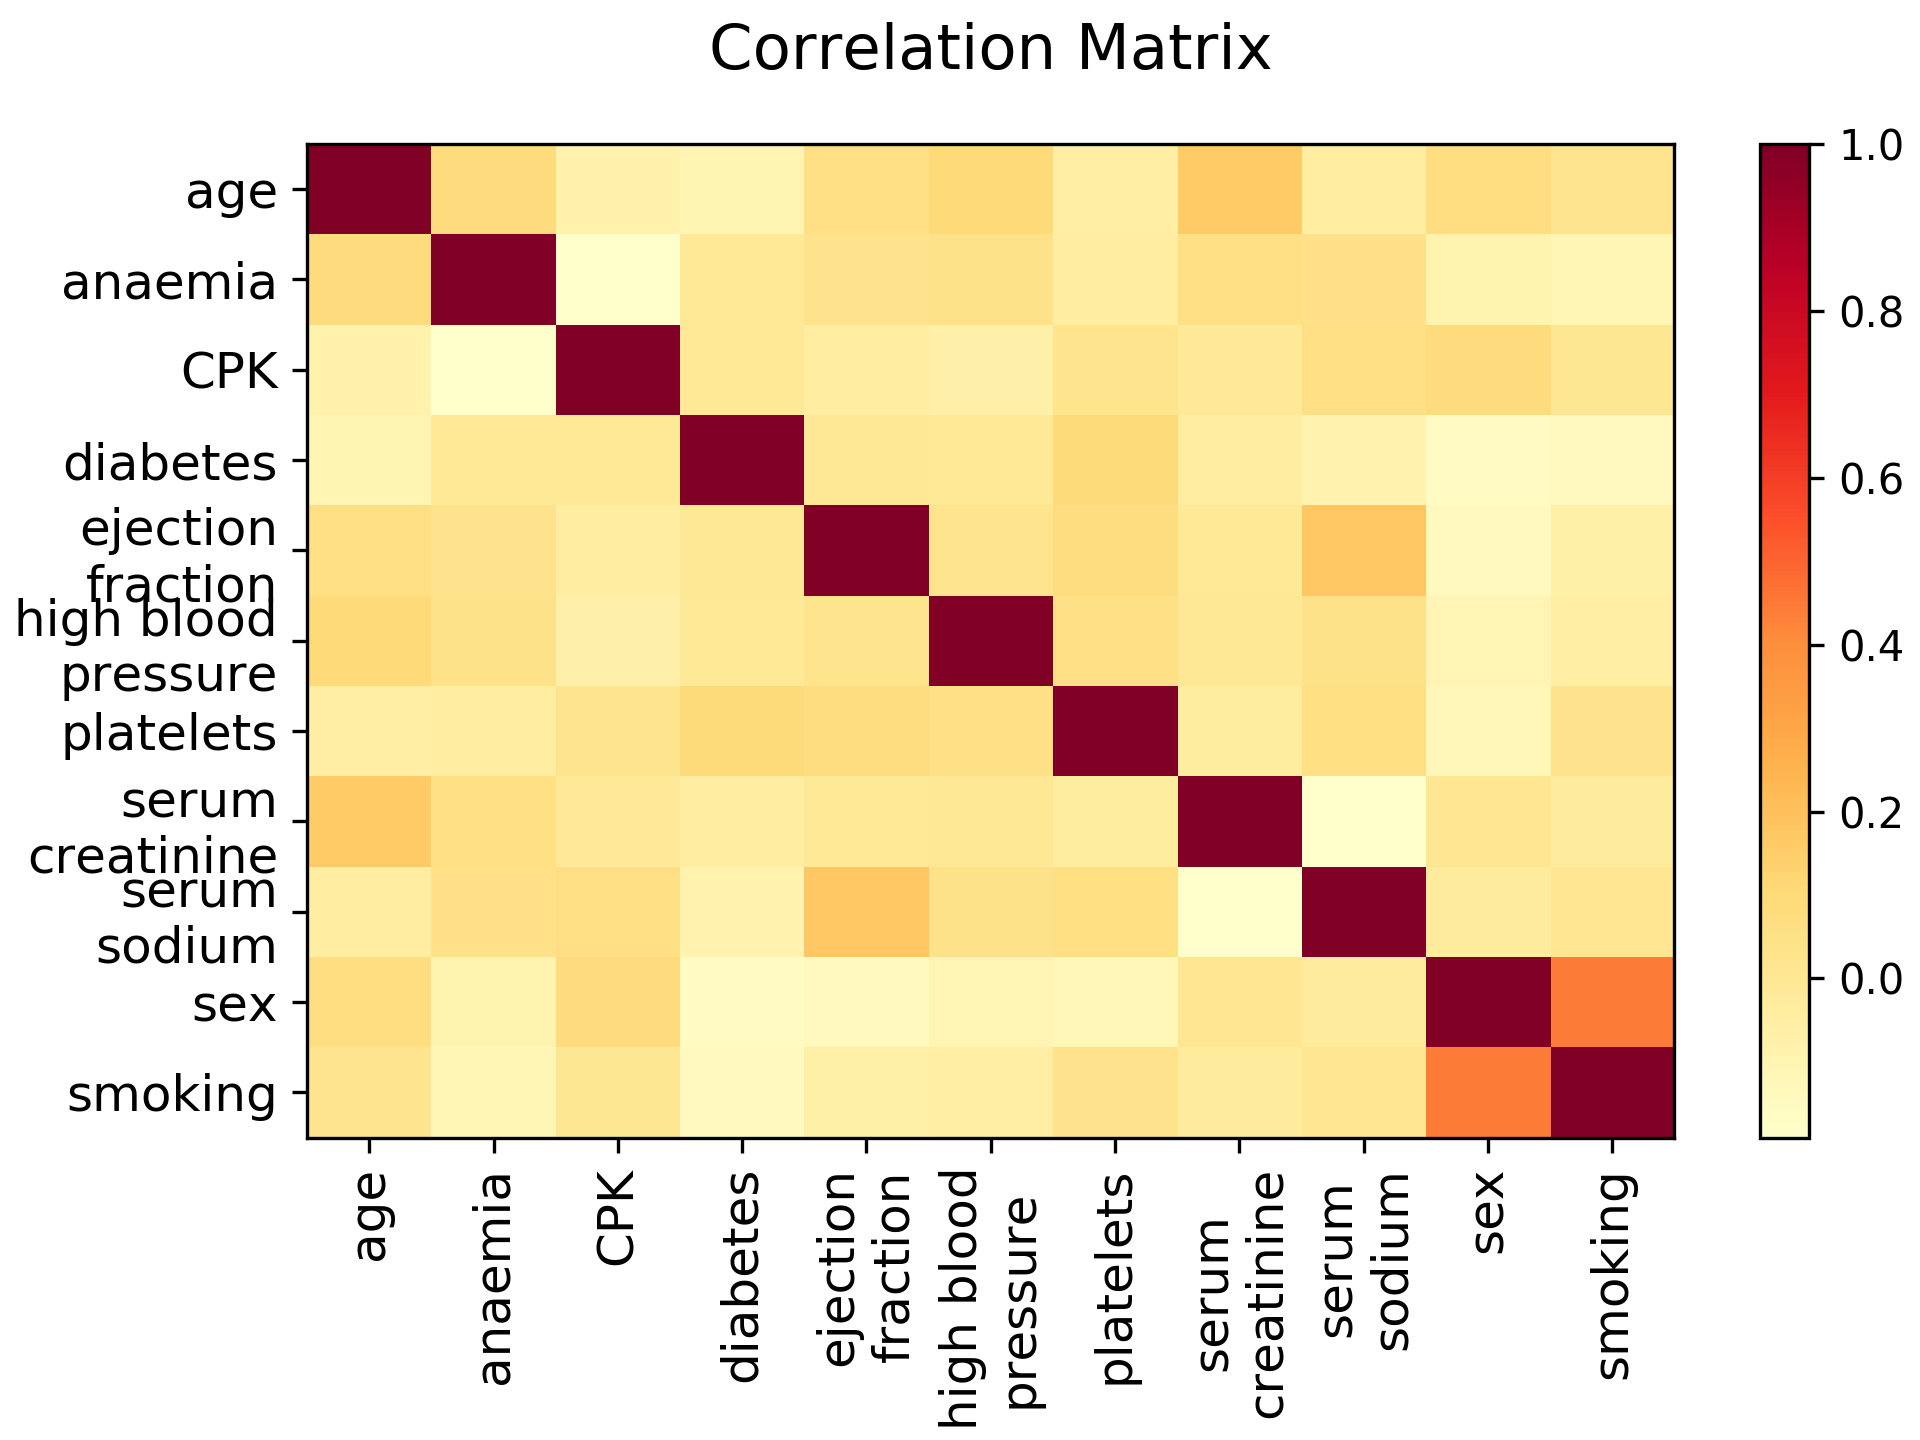
\includegraphics[width=0.5\textwidth]{../Figures/correlation_matrix.png}
	\caption{Correlation matrix of the heart disease dataset.}
	\label{corr}
\end{figure}

\begin{table*}
\centering
\begin{tabular}{|l|l|l|}
\hline
\multicolumn{1}{|c|}{\textbf{Feature}} & \multicolumn{1}{c|}{\textbf{Explanation}} & \multicolumn{1}{c|}{\textbf{Unit}} \\ \hline
Age & Age of patient & Years \\ \hline
Anaemia & Whether the patient is anaemic & Boolean \\ \hline
Creatinine phosphokinase & Amount of CPK in the blood & mcg/l \\ \hline
Diabetes & Whether the patient is diabetic & Boolean \\ \hline
Ejection fraction & \begin{tabular}[c]{@{}l@{}}Amount of blood leaving the heart during \\ each contraction\end{tabular} & Percentage \\ \hline
High blood pressure & Whether the patient is hypertensive & Boolean \\ \hline
Platelets & Amount of platelets in the blood & kiloplatelets/ml \\ \hline
Serum creatinine & Amount of serum creatinine in the blood & mg/dl \\ \hline
Serum sodium & Amount of serum sodium in the blood & mEq/l \\ \hline
Sex & Gender of patient & Boolean \\ \hline
Smoking & Whether the patient is a smoker & Boolean \\ \hline
Time & Duration of follow-up period & Days \\ \hline
Death event & \begin{tabular}[c]{@{}l@{}}Whether the patient perished during \\ follow-up period\end{tabular} & Boolean \\ \hline
\end{tabular}
\caption{Explanation of features in the heart failure dataset. }
\label{features}
\end{table*}


\subsection{Logistic regression}
Logistic regression is a standard classification method. In this project, the logistic regression method will only be presented for binary problems with classes $y=0$ and $y=1$. The basic idea is to perform linear regression on a logistic transformation of the probability $p$ of observing $y=1$: 
\begin{equation}\ln \frac{p}{1-p}=\beta_0+\beta_1x_1+\dots + \beta_k x_k, \end{equation}
where $k$ is the total number of input features. If we write $\vb{x}=(x_1,\dots,x_k)$ and $\boldsymbol{\beta}=(\beta_1,\dots,\beta_k)$ we can solve for $p$ and get 
\begin{equation}p=\frac{e^{\beta_0+\boldsymbol{\beta}^T\vb{x}}}{1 +  e^{\beta_0+\boldsymbol{\beta}^T\vb{x}}}\end{equation}
For a particular observation $\vb{x_i}$ we predict $y_i=1$ if $p>\frac{1}{2}$ and $y_i=0$ otherwise.  \\[2mm]
In order to determine the regression coefficients $\beta_0$ and $\boldsymbol{\beta}$ we aim to minimise the cross entropy cost function\cite{lecturenotes4}: 
\begin{equation}C(\beta_0, \boldsymbol{\beta})=-\sum_{i=1}^N \Big(y_i(\beta_0+\boldsymbol{\beta}^T\vb{x_i})-\ln{}(1+e^{\beta_0+\boldsymbol{\beta}^T\vb{x_i}})\Big)\end{equation}
One may derive cross entropy from the maximum likelihood method by considering the log likelihood (specifically, minimising the negative log likelihood). The cost function is typically minimised using gradient descent methods, which requires the derivative of cross entropy: 
\begin{align}
	\pdv{C(\beta_0, \boldsymbol{\beta})}{\beta_0}&=-\sum_{i=1}^N\Big(y_i-\frac{e^{\beta_0+\boldsymbol{\beta}^T\vb{x_i}}}{1+e^{\beta_0+\boldsymbol{\beta}^T\vb{x_i}}}\Big),\\
	\pdv{C(\beta_0, \boldsymbol{\beta})}{\boldsymbol{\beta}}&=-\sum_{i=1}^N\Big(y_i\vb{x_i} - \vb{x_i}\frac{e^{\beta_0+\boldsymbol{\beta}^T\vb{x_i}}}{1+e^{\beta_0+\boldsymbol{\beta}^T\vb{x_i}}}\Big)
\end{align}	
The gradient descent methods are handled internally by \texttt{sklearn}. A more detailed description was presented in Project 2. \cite{project2} \\[2mm]
In addition to cross entropy, it is common to add an $L^2$-penalty term in order to regularise the size of the coefficients. This is implemented by adding the term $\lambda\norm{\boldsymbol{\beta}}^2$ to the cost function. The penalty, $\lambda$, must be determined experimentally. One option is to cross validate the performance of models of different penalties (see section \ref{cv}).

\subsection{Decision trees and random forests}
\subsubsection{Decision trees}
In a decision tree, a data set is divided and arranged into regions by recursive binary splitting. \cite{ISL} Decision trees get their name from their tree-like structure consisting of nodes connected by branches. Each node represents a binary split in a single feature in the data set, and each branch represents the result of the split. The initial node is called the root node and the final nodes, where we find the prediction, are known as leaves. \\[2mm]
For a node $m$ that represents a region $R_m$ containing $N_m$ observations, the proportion of observations from class $k$ is given by \cite{ESL}
\begin{equation} p_{mk}=\frac{1}{N_m}\sum_{x_i \in R_m}I(y_i=k)\end{equation}
A decision tree can be trained using for instance the classification and regression tree (CART) algorithm. At each node $m$ the CART algorithm assigns the following cost function to each feature and threshold pair ($k$, $t_k$) \cite{lecturenotes1}:
\begin{equation}C(k, t_k)=\frac{m_{\text{left}}}{m}G_{\text{left}}+\frac{m_{\text{right}}}{m}G_{\text{right}}\end{equation}
where $G_{\text{left/right}}$ is a measure of the impurity of the left and right subsets respectively, while $m_{\text{left/right}}$ is the number of points in each subset. The CART algorithm minimises the total cost function (sum of cost from each node) by minimising $C(k, t_k)$ at each node.
\newpage
The impurity of a subset is a measure of the quality of the split. There are several ways of measuring node impurity, we have opted to use the gini index, given by \cite{ESL}
\begin{equation} G_m=\sum_{k=1}^{K}p_{mk}(1-p_{mk})\end{equation}
In this project we employ the \texttt{sklearn} implementation \cite{scikit-learn} of decision trees via their implementation of random forest. 

\subsubsection{Random forests}
The random forest is an ensemble of decision trees. Each tree is an independent classifier working on a bootstrap sample of the data and the forest prediction is the average prediction of all the trees based on a majority vote. \cite{lecturenotes3} In contrast to ordinary decision trees, the trees in a random forest are trained such that each split is based on a random subset of the input variables. \cite{ESL} \\[2mm]
The most important parameter to consider when creating a random forest is the number of trees, which should be sufficiently large (increasing the number of trees beyond this threshold does not improve the model). In addition, the maximum depth of each tree and the number of features used in each split must be predetermined. 


\subsection{Support vector machines}
The following is heavily based on Hastie et al's book \cite{ESL} and James et al's book \cite{ISL}. 
\subsubsection{The formalism of support vector machines}
The main idea of support vector machines (SVMs) is to create a boundary, known as a hyperplane, in feature space that separates data points of different classes. A hyperplane in a $p$-dimensional space is an affine subspace of dimension $p-1$, given by 
\begin{equation}\vb{x}^T\vb{w}+b=0,\end{equation} 
where $\vb{x}$ is a position vector in the space, $\vb{w}$ is a parameter vector with $\norm{\vb{w}}=1$ describing the hyperplane and $b$ is the intercept term. Points $\vb{x}$ in the data set can be classified into two distinct regions based on wether they are above or below the hyperplane, which is determined by the sign of $\vb{x}^T\vb{w}+b$. Thus for an observation $\vb{x_i}$ we classify the data point as $y_i=\pm1$. The aim of the SVM is to maximise the distance between the hyperplane and the points belonging to each class such that the binary classes are separated by the hyperplane. \\[2mm]
For convenience, we define $f(\vb{x}) = \vb{x}^T\vb{w}+b$ such that the hyperplane is given by $f(\vb{x})=0$. Since $y_i=1$ whenever $f(\vb{x_i}>0$ and $y_i=-1$ whenever $f(\vb{x_i}<0$ we must have 
\begin{equation}y_i f(\vb{x_i})>0\quad \forall i\end{equation}
The idea of SVM is to find the greatest margin $M>0$ such that 
\begin{equation}\label{constraint1} y_if(\vb{x_i})\geq M, \quad i=1,\dots, N.\end{equation}
It is, however, unreasonable to assume that the points of each class are well separated by a hyperplane with no overlap. This can be handled by introducing a slack variable $\boldsymbol{\xi}=(\xi_1, \xi_2, \dots, \xi_N)$ that allows for some points to be on the wrong side of the boundary. The constraint of equation \ref{constraint1} can now be modified to 
\begin{equation} y_if(\vb{x_i})\geq M(1-\xi_i)\quad \forall i,\end{equation}
with $\xi_i\geq0$ and $\sum_{i=1}^{N}\xi_i\leq K$, where $K$ is some constant. When $\xi_i > 1$ we have a misclassification. Therefore, by ensuring $\sum_{i=1}^{N}\xi_i\leq K$, the number of allowed misclassifications is automatically limited by $K$. If we let $M=1/\norm{\vb{w}}$ and let $\norm{\vb{w}}$ vary, we may rephrase the constraint problem as 
\begin{equation} \min\norm{\vb{w}}\qq{subject to}\begin{cases}y_i f(\vb{x_i})\geq 1-\xi_i \ \forall i, \\ \xi_i\geq 0, \sum\xi_i\leq K\end{cases}\end{equation}
In order to solve the constraint problem we must formulate it as a Lagrangian constraint problem. We begin by rephrasing the above condition to 
\begin{align} 
	&\min \frac{1}{2}\norm{\vb{w}}^2 + C\sum_{i=1}^N \xi_i \nonumber \\
	&\text{subject to} \ \xi_i\geq0, y_i f(\vb{x_i}) \geq 1-\xi_i\ \forall i
\end{align}
The corresponding Lagrange function to this constraint problem is 
\begin{align}
	L_P = &\frac{1}{2}\norm{\vb{w}}^2 + C\sum_{i=1}^N \xi_i\nonumber \\
	&-\sum_{i=1}^N\alpha_i[y_if(\vb{x_i})-(1-\xi_i)]-\sum_{i=1}^N\mu_i\xi_i \label{den_lange}
\end{align}
where $\alpha_i$ and $\mu_i$ are the Lagrange multipliers. Computing the derivatives of $[y_if(\vb{x_i})-(1-\xi_i)]$ and $[\xi_i]$ with respect to $\vb{w}$, $b$ and each $\xi_i$ yields for all $i$: 
\begin{align}
	\vb{w}&=\sum_{i=1}^N\alpha_i y_i \vb{x_i}\\
	0&=\sum_{i=1}^N\alpha_i y_i\\
	\alpha_i &= C-\mu_i
\end{align}
Substituting these into equation \ref{den_lange} we get
\begin{equation} L_D=\sum_{i=1}^N \alpha_i-\frac{1}{2}\sum_{i=1}^N\sum_{j=1}^N \alpha_i\alpha_jy_iy_j \vb{x_i}^T\vb{x_j}\end{equation}
This equation is maximised for $0\leq\alpha_i\leq C$ and $\sum_{i=1}^N\alpha_iy_i=0$, in addition to the Karush-Kuhn-Tucker conditions: 
\begin{align}
	\alpha_i [y_if(\vb{x_i})-(1-\xi_i)]&=0, \\
	\mu_i\xi_i &= 0, \\
	y_if(\vb{x_i})-(1-\xi_i)&\geq 0,
\end{align}
for $i=1,\dots, N$. This constraint problem can be solved using convex quadratic programming methods, which in this project is handled internally by \texttt{sklearn}.

\subsubsection{Kernel methods}
So far we have only considered linear boundaries in the feature space. However, the SVM can be made more flexible by allowing different sets of basis functions. By introducing basis transformations $h(\vb{x_i})=(h_1(\vb{x_i}), h_2\vb{x_i},\dots, h_M(\vb{x_i}))$ for $i=1,\dots,N$, we may follow the same procedures as before using $h(\vb{x_i})$ as points in the feature space, i.e. replace $\vb{x_i}$ with $h(\vb{x_i})$. Going through the process yields the following Lagrange function:
\begin{align}
	L_D =\sum_{i=1}^N\alpha_i - \frac{1}{2}\sum_{i=1}^N\sum_{j=1}^N \alpha_i\alpha_jy_iy_j \langle h(\vb{x_i}), h(\vb{x_j})\rangle
\end{align}
Because this equation only depends on the inner product of $h(\vb{x_i})$ and $h(\vb{x_j})$, its suffices to specify the kernel function
\begin{equation}K(x, x')=\langle h(x), h(x')\rangle. \end{equation} 
For this project, the following kernels are implemented: 
\begin{align}
	\text{Polynomial kernel:}\ &K(x, x') = (1+\langle x,x'\rangle )^d \\
	\text{Radial kernel:}\ &K(x, x') = \exp(-\gamma \norm{x, x'}^2),
\end{align}
where $\gamma$ is a parameter. We use the \texttt{sklearn} default value. 

\subsection{Evaluating the models} \label{cv}
The standard way of evaluating classifiers (and any supervised machine learning algorithm in general) is to divide the data set at random into a a training set and testing set. The training set is used to prepare the classifiers, which are then evaluated using the testing set. Typically, most of the data is used for training. In order to compare the classifiers, the accuracy classification metric is used. Accuracy is defined as the number of correct predictions normalised by number of samples:
\begin{equation}\label{acc}\text{Accuracy}(y, \hat{y})=\frac{1}{N}\sum_{i=0}^{N-1}1(\hat{y_i}=y_i)\end{equation}
where N is the number of samples, $y$ is the observed response and $\hat{y}$ is the predicted. \\[2mm]
The data set used in this project contains only 299 points, which means that the testing set is very sensitive to the random selection. In order to get a good estimate of the accuracy we implement $K$-fold cross validation. The main idea is to split the data set into $K$ folds (subsets) which are then iteratively used as testing sets (using the remaining points as training data). The algorithm is as follows: 
\begin{algorithm}[H]
	\caption{K-fold Cross Validation}
	\begin{algorithmic}[1]
		\State Split data into $K$ folds at random  
		\For {$k = 1,2, \dots, K$}
			\State The $k$th set is used as testing data and the remaining points are used as training data
			\State The model is fitted and validated, the accuracy is calculated 
		\EndFor
		\State The average and standard deviation of the calculated accuracies are computed
	\end{algorithmic}
\end{algorithm}
The average accuracy is used as an estimate of the true accuracy, with the standard deviation as an estimate of the uncertainty. In the data set used in this project, there are 203 patients that survived and 96 patients that died. This means that a randomly selected fold will typically contain more surviving patients than dead patients. We might even have a situation where a fold contains no dead patients at all. In order to ensure that both classes are represented in every fold, we use a stratified version of $K$-fold cross validation that splits the data such that each fold contains roughly the same percentage of dead patients. \\[2mm]
In this project, we use cross validation as a tool for optimising the models' parameters. In the logistic regression case, we use cross validation to determine the optimal penalty $\lambda$. For random forests we use cross validation to determine a sufficient number of trees, and the best combination of tree depth and number of features per split. Finally, for support vector machines, we use cross validation to determine the optimal cost $C$ for each kernel. 

\subsection{Feature selection}
The basic idea of feature selection is to determine what features have the greatest impact on a classification model. This will provide an indication of wether the input features are related to the outcome. In our case, we want to determine what medical records are most correlated with survival in order to gain a better understanding of the underlying mechanisms of heart failure deaths. \\[2mm]
As opposed to logistic regression and support vector machines, random forests have an inherent feature selection ability based on averaging the importance of the features in each tree. In particular, the feature importance computes the total gain in the gini index of each tree when a feature is removed completely from the forest. \\[2mm]
A general-purpose method for feature selection is recursive feature elimination (RFE). RFE is based on a selection criterion that identifies the least important feature in the model. The idea is to measure the performance of the full model and recursively remove the feature that is determined to be least important via the selection criterion. For random forests, the selection criterion is based on the inherent feature importance measure. There is no equivalent natural way of determining the selection criterion for logistic regression and support vector machines. A common choice is to rank the features according to the square of their coefficients. In this project, we will average the performance at each step over 100 repetitions. RFE selects the most important features by choosing the smallest set of features for which the average performance is within the confidence interval of the performance of the full model. In this project, the confidence interval is taken as within one standard deviation of the average accuracy of the full model. 
\section{Results}
\subsection{Model optimisation}
Figure \ref{CV_LR} shows the 5-fold cross validated accuracies for different penalties in the logistic regression model. Overall, there are no significantly large improvements to be made by tuning the penalty. However, there is a local maximum at $\lambda=0.1$, which is the value we will use in the feature selection process. While tuning the parameter does not significantly improve the model, a large penalty ($\lambda \geq 10^2$) limits the accuracy to approximately 0.7. Figure \ref{CM_LR} shows the confusion matrix of the logistic regression model when using $\lambda=0.1$. We see that the largest contribution to the accuracy comes from surviving patients (0) that are correctly labeled. From the lower row, we see that most dead patients are predicted to survive. Using the optimal penalty $\lambda=0.1$, the logistic regression model achieves an accuracy of $0.746\pm0.041$ (5fold cross validated). \\[2mm]
\begin{figure}[b]
	\centering
	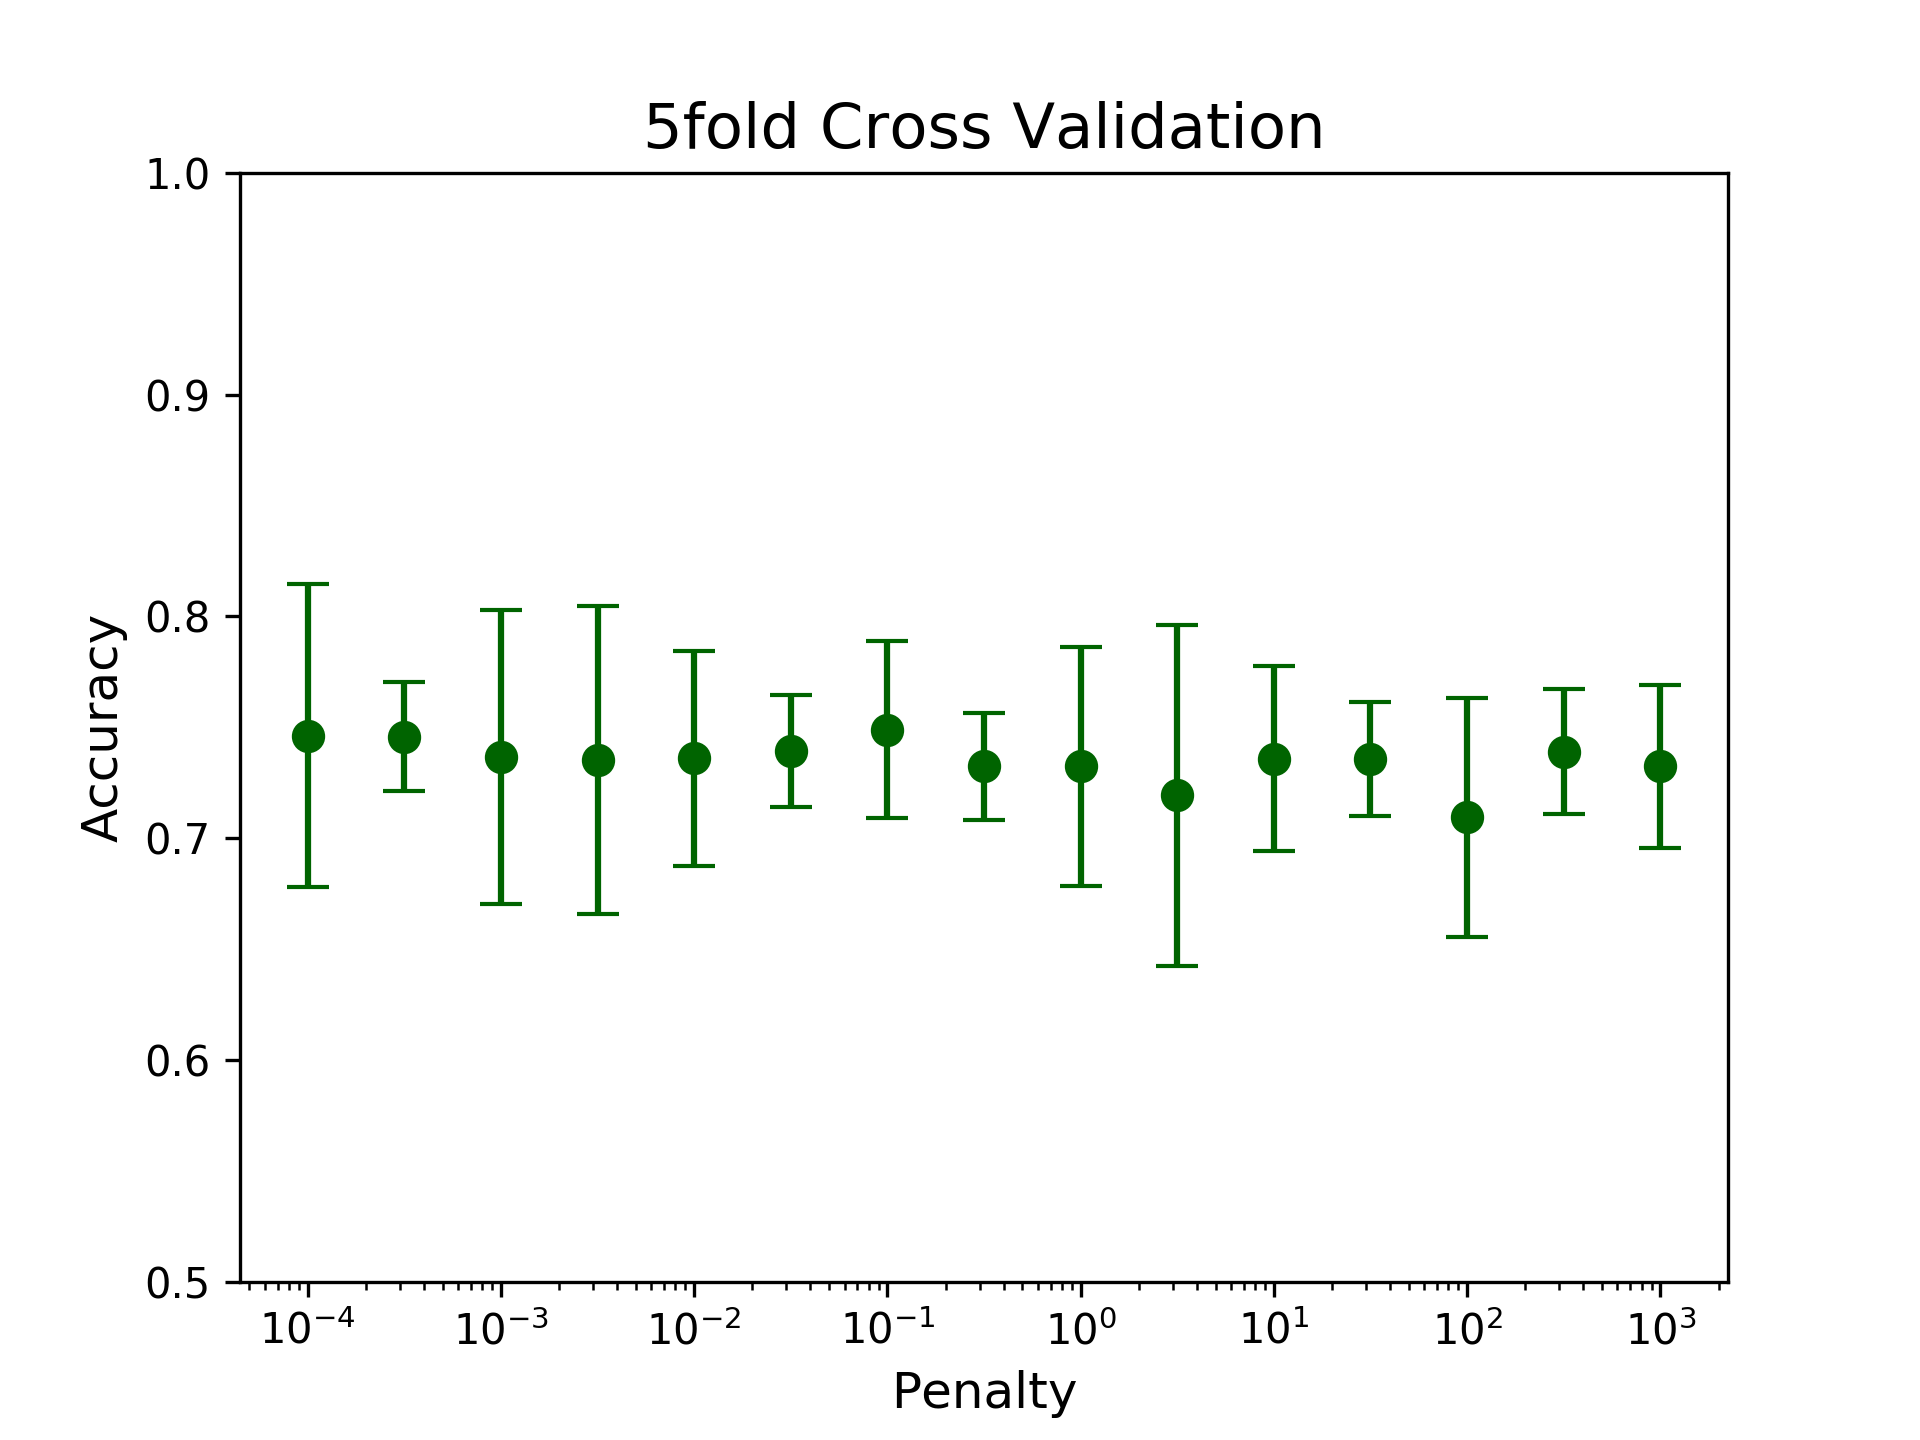
\includegraphics[width=0.45\textwidth]{../Figures/5fold_CV_LR_penalties.png}
	\caption{Cross validated accuracies of different penalties for logistic regression. }
	\label{CV_LR}
\end{figure}
\newpage
Figure \ref{CV_RFC} shows the 5-fold cross validated accuracies for different number of trees in a random forest model. There is no significant improvement to the accuracy for a number of trees higher than 50, and this is the number of trees we will take as being sufficient. Figure \ref{hyperparam_RFC} shows the 5-fold cross validated accuracies of different combinations of maximum tree depth and number of features at each split for a random forest model with 50 trees. There is no clear pattern for determining the optimal combination, although the best result was achieved with a maximum depth of 15 and maximally 7 features per tree. Figure \ref{CM_RFC} shows the confusion matrix for the best random forest model. Similar to the logistic regression confusion matrix, the random forest confusion matrix shows that the model is worse at predicting patient deaths compared to survivals. Using the optimal choice of a maximum tree depth of 15 and a maximum of 7 features per tree, the random forest achieves an accuracy of $0.756\pm0.022$.
\begin{figure}[h!]
	\centering
	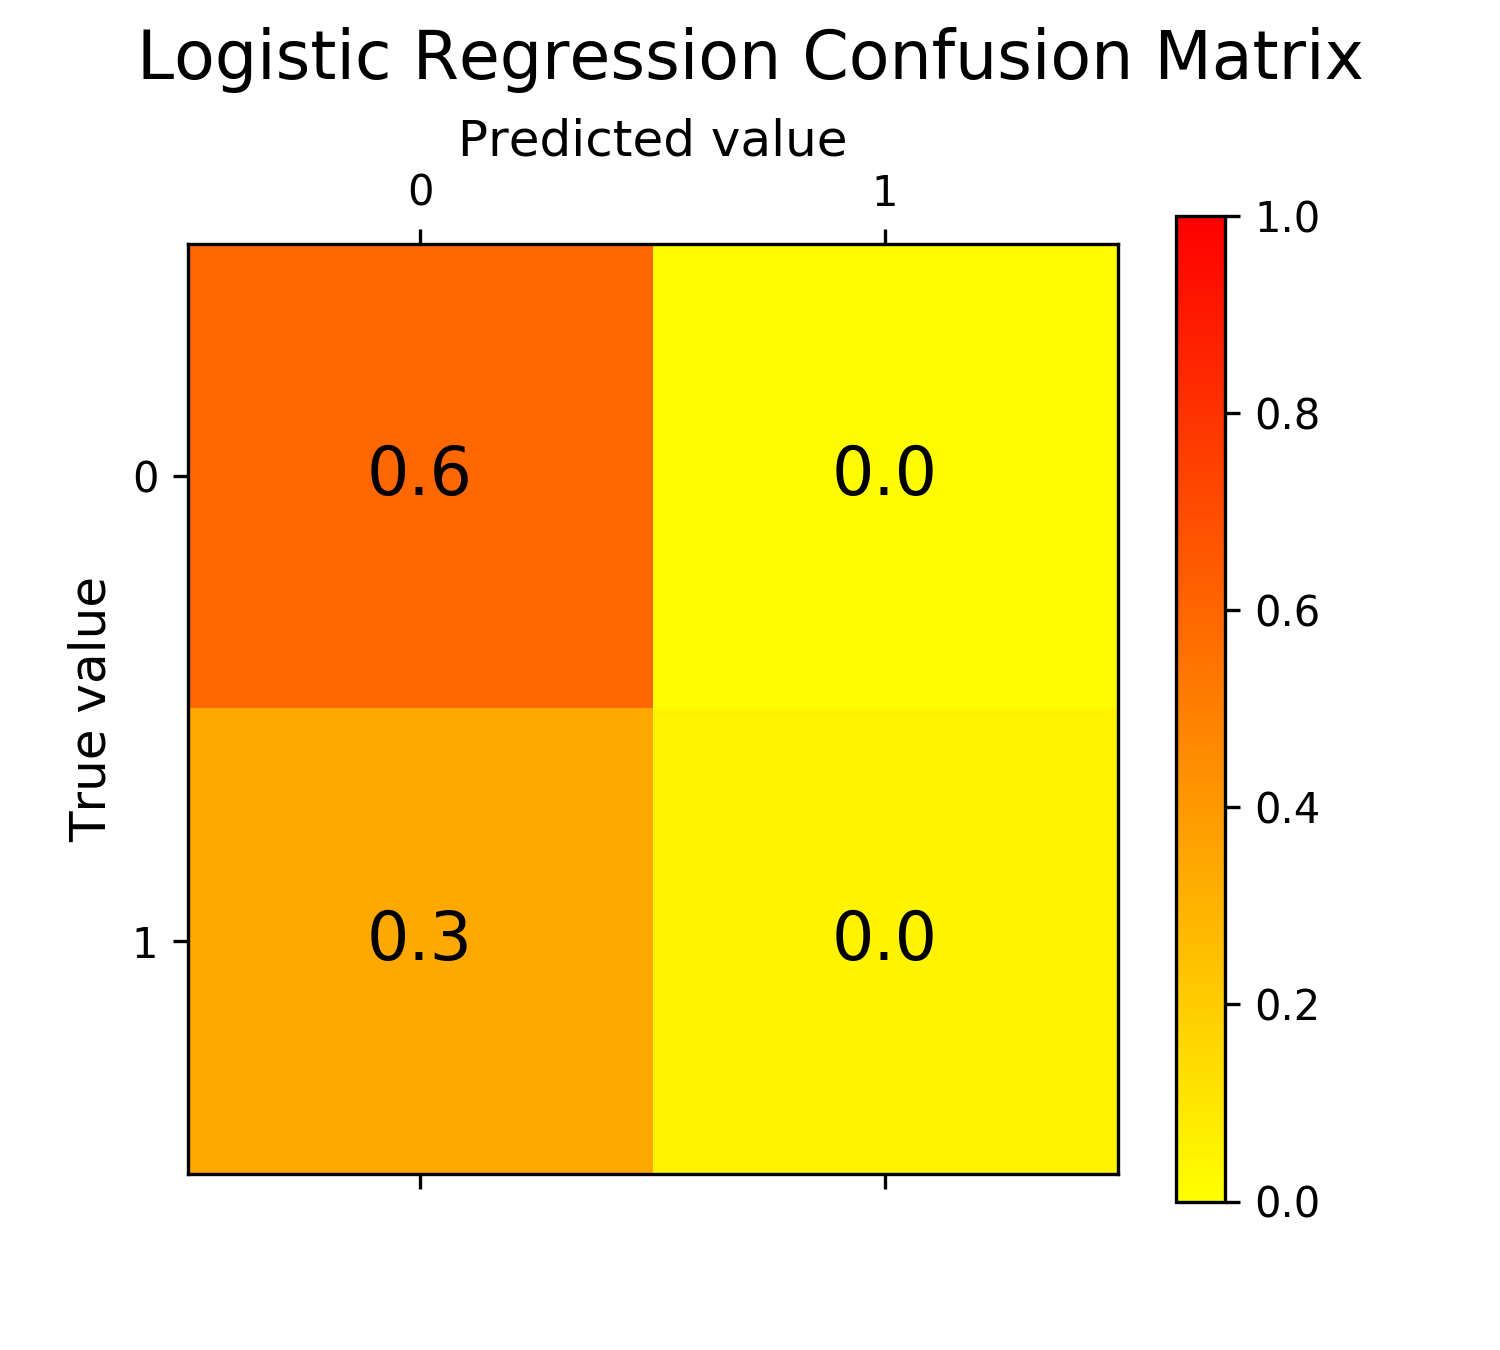
\includegraphics[width=0.42\textwidth]{../Figures/CM_LR.png}
	\caption{Confusion matrix for best logistic regression model.}
	\label{CM_LR}
\end{figure}
\begin{figure}[h!]
	\centering
	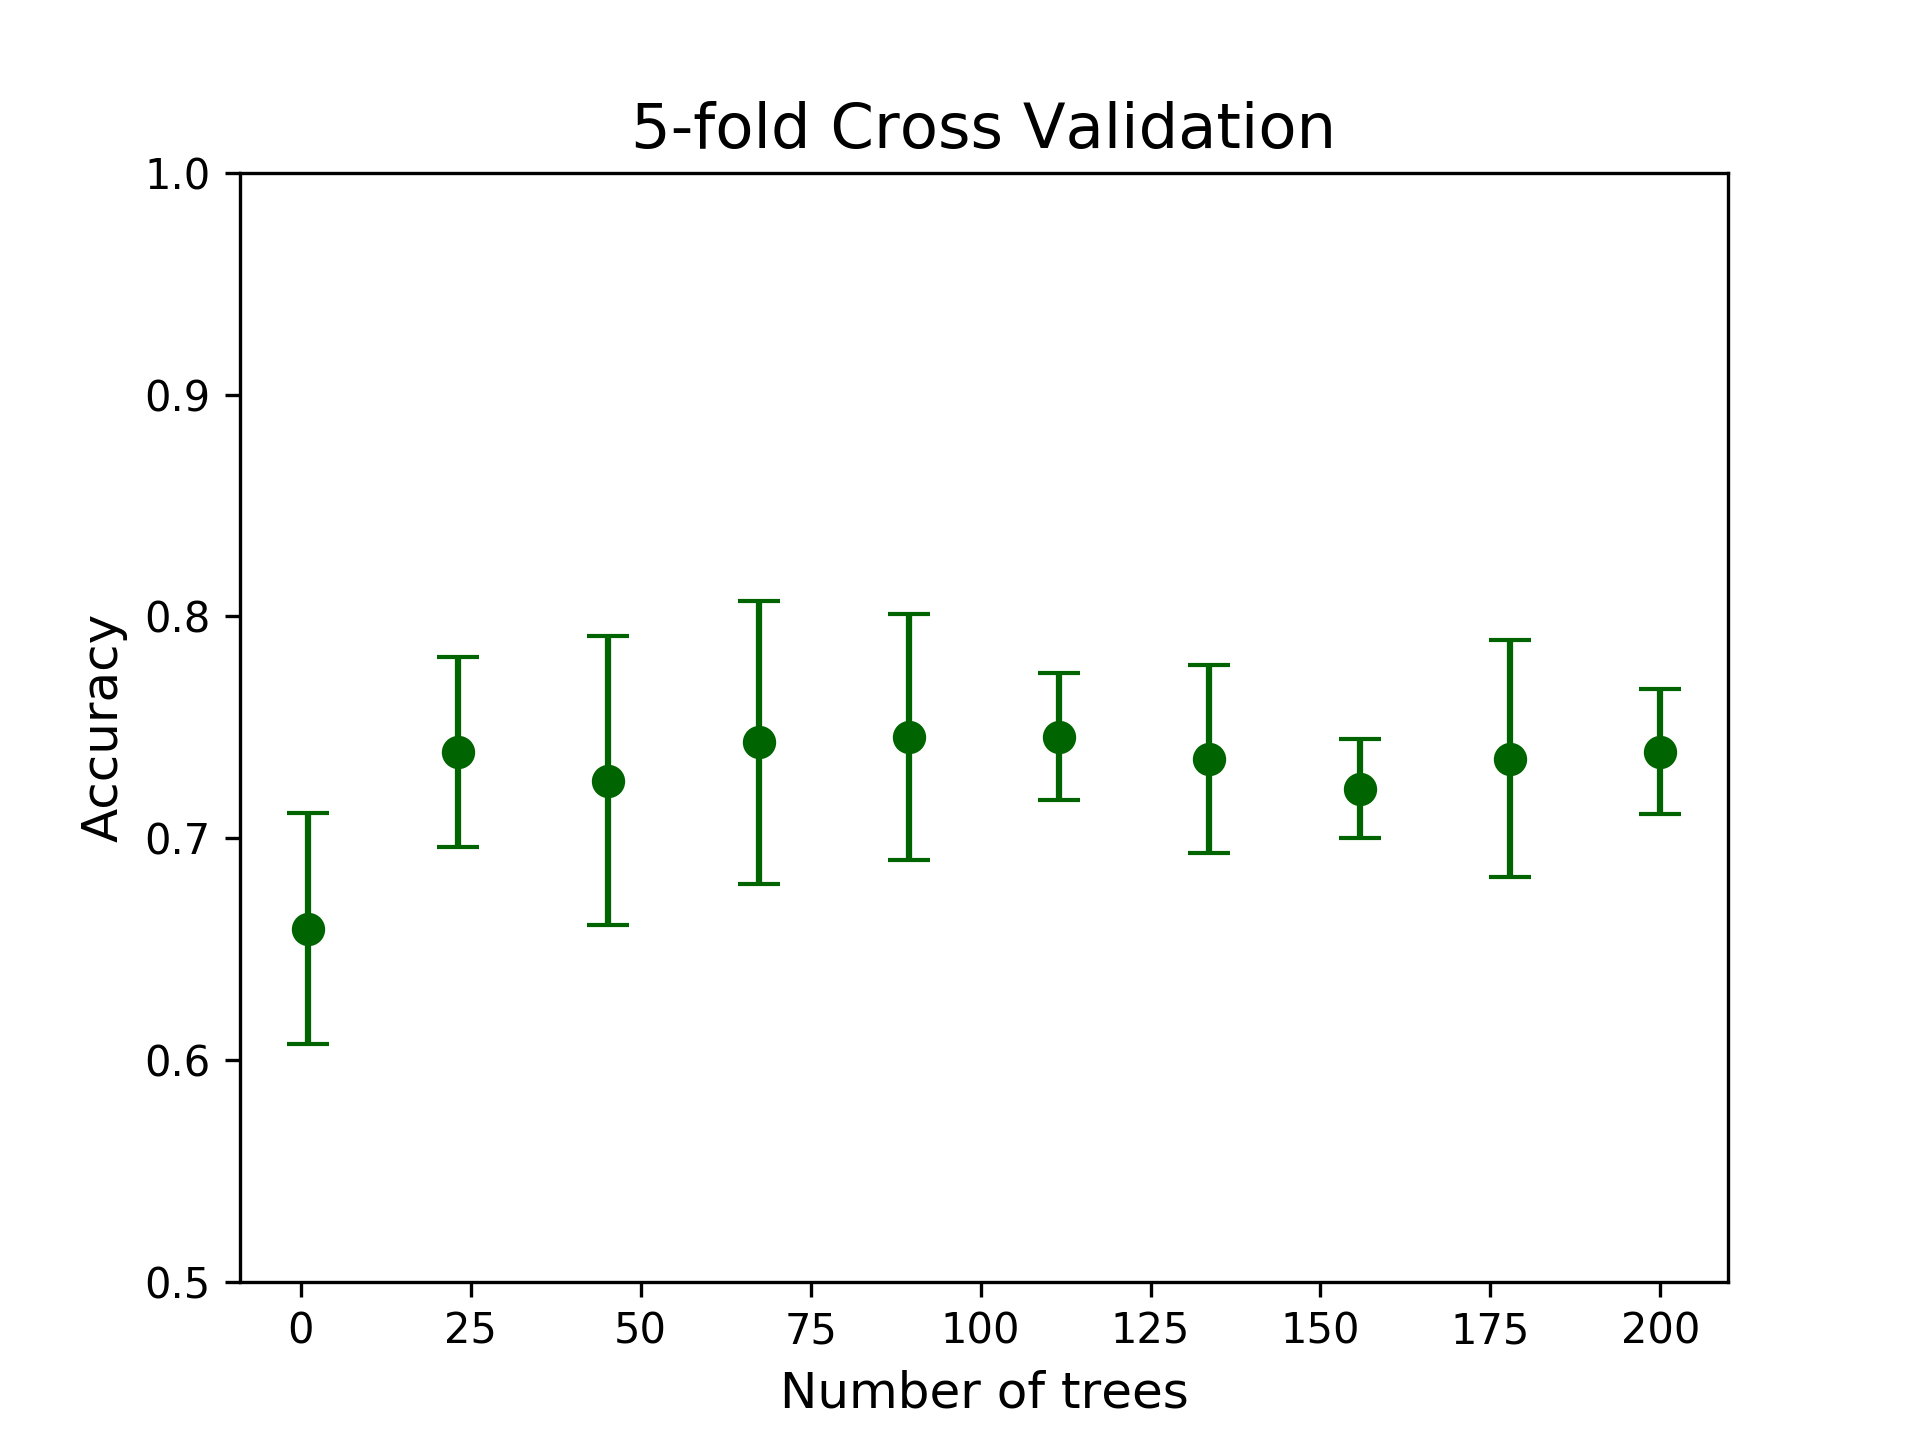
\includegraphics[width=0.42\textwidth]{../Figures/5fold_CV_RFC_ntrees.png}
	\caption{Cross validated accuracies for different number of trees in a random forest.}
	\label{CV_RFC}
\end{figure}
\newpage 
\begin{figure}[h!]
	\centering
	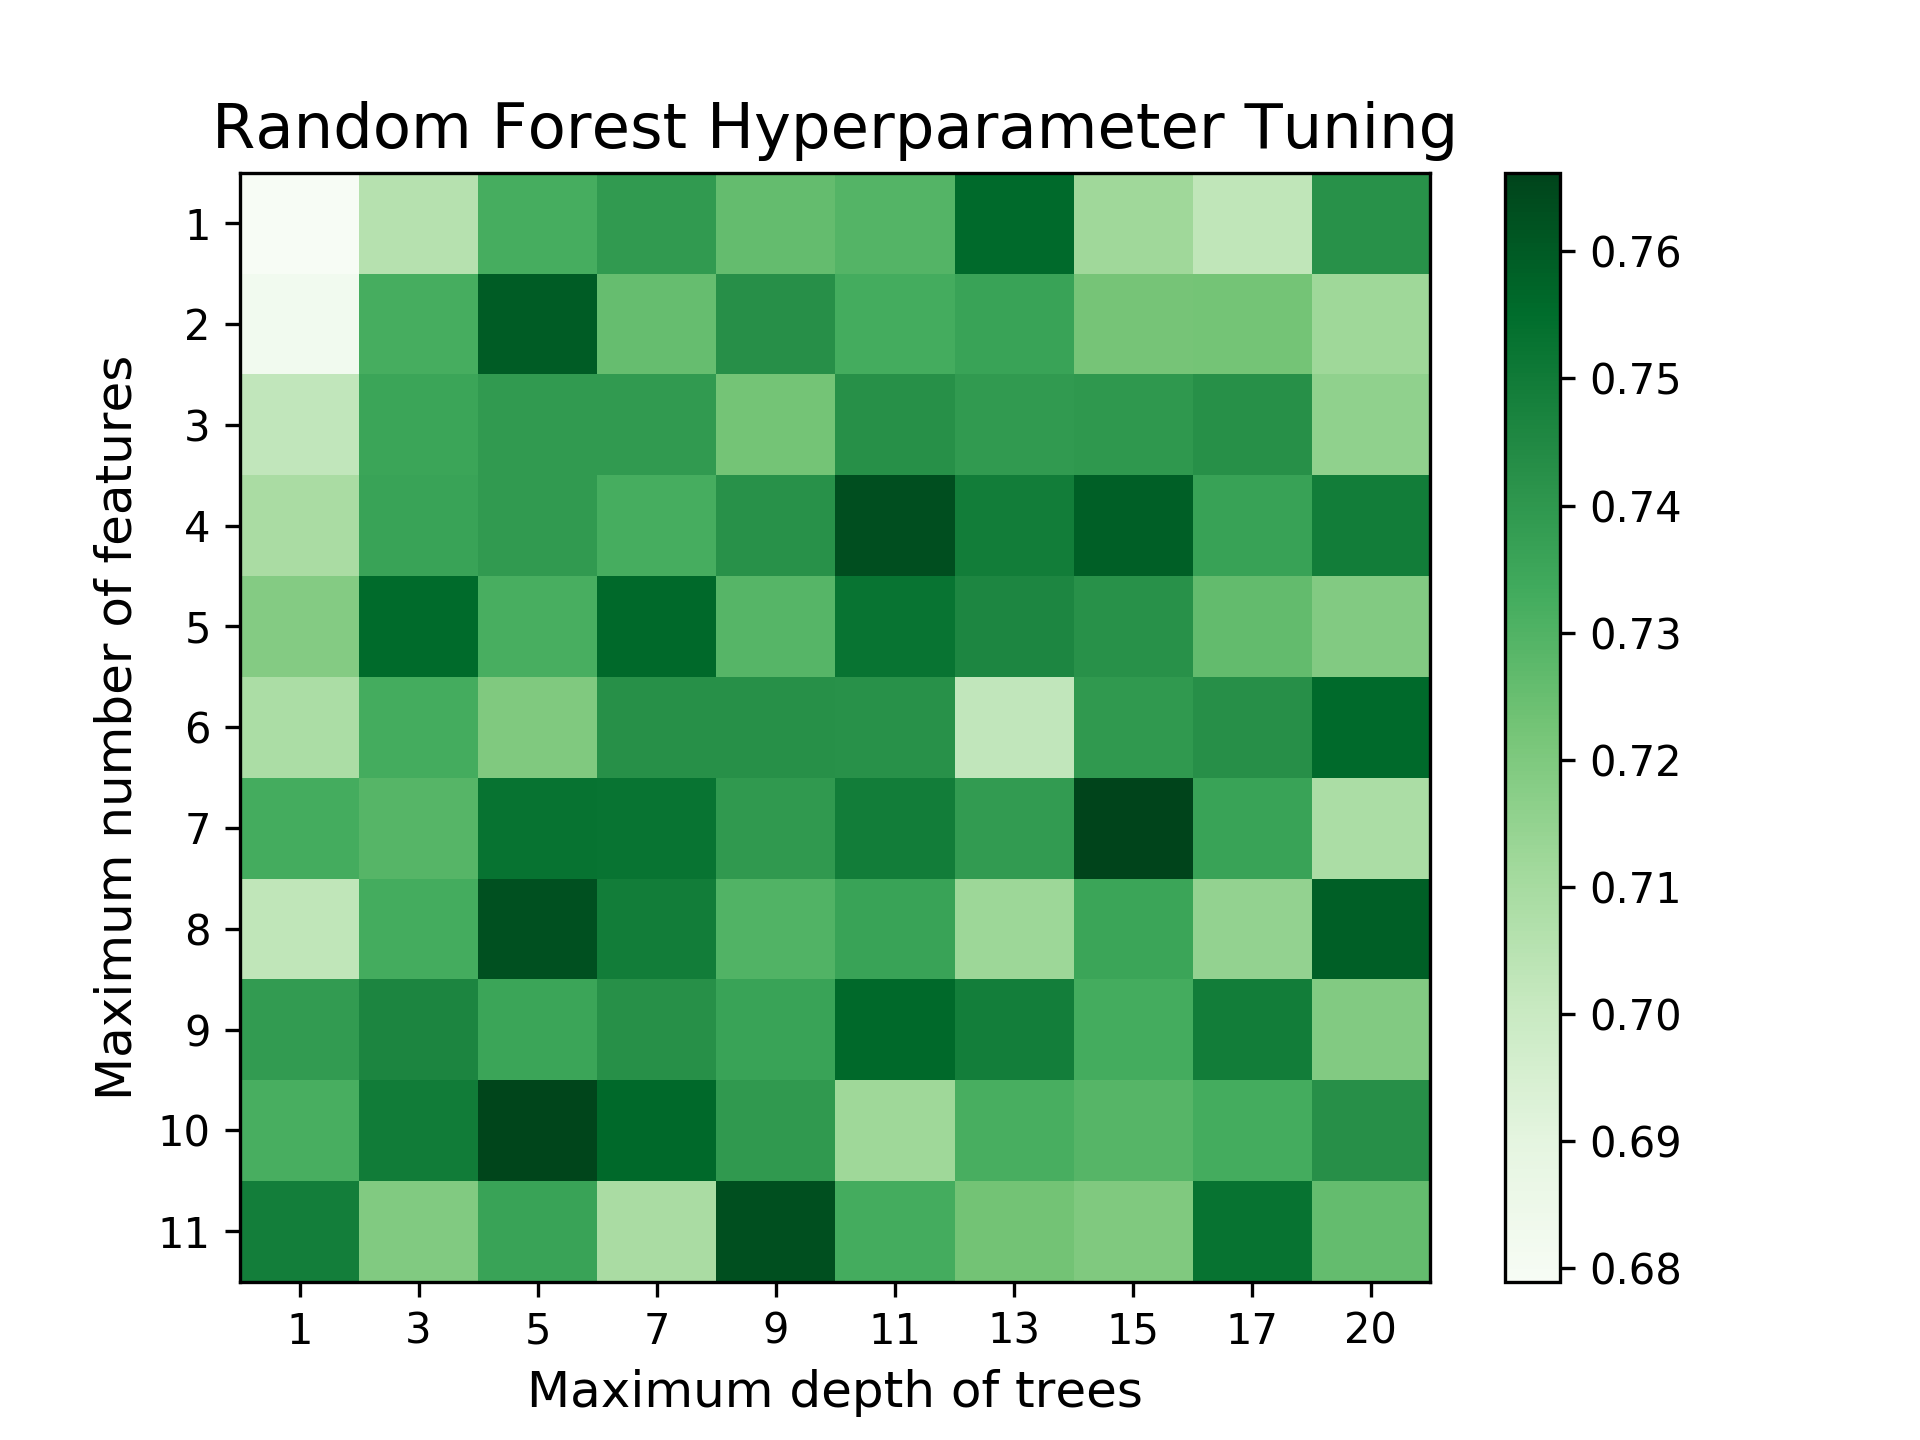
\includegraphics[width=0.42\textwidth]{../Figures/hyperparameter_tuning_RFC.png}
	\caption{Cross validated accuracies for combinations of hyperparameters for random forest.}
	\label{hyperparam_RFC}
\end{figure}
\begin{figure}[h!]
	\centering
	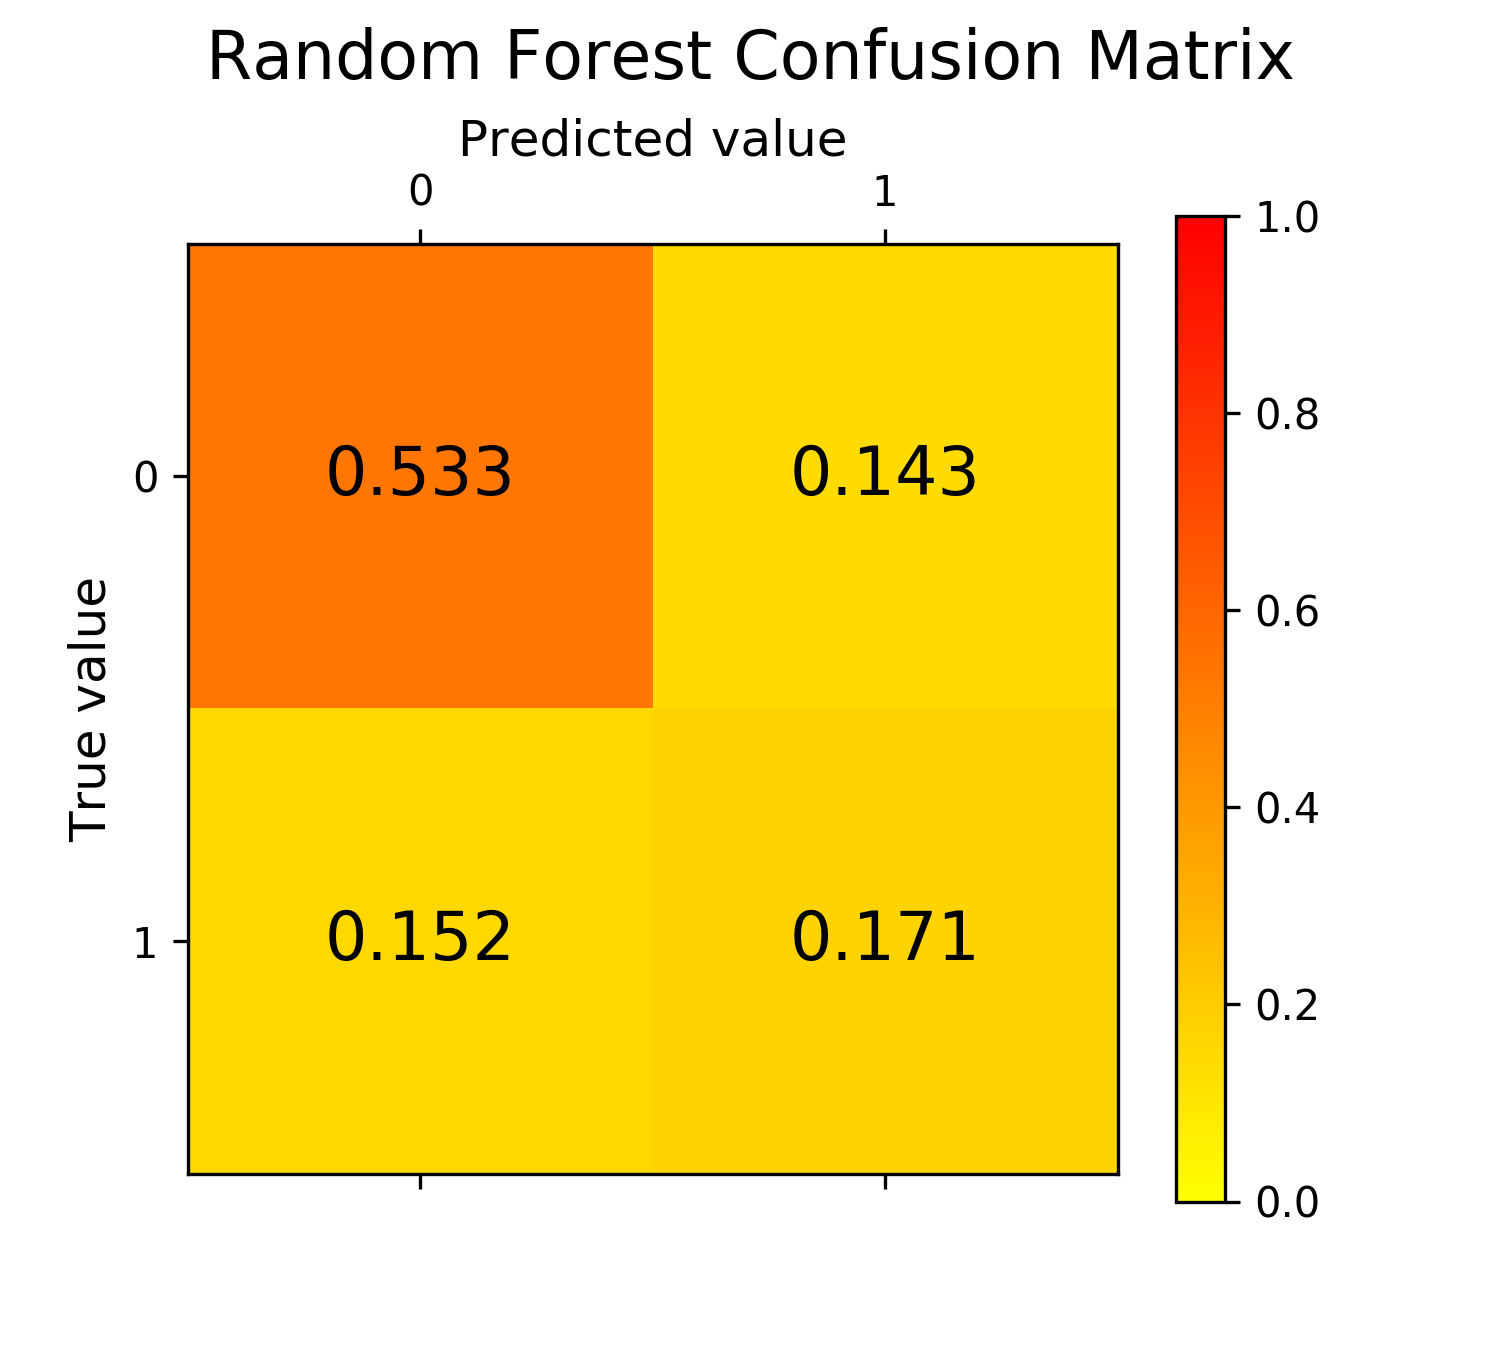
\includegraphics[width=0.42\textwidth]{../Figures/CM_RF.png}
	\caption{Confusion matrix for best random forest model.}
	\label{CM_RFC}
\end{figure}
\begin{figure}[h!]t
	\centering
	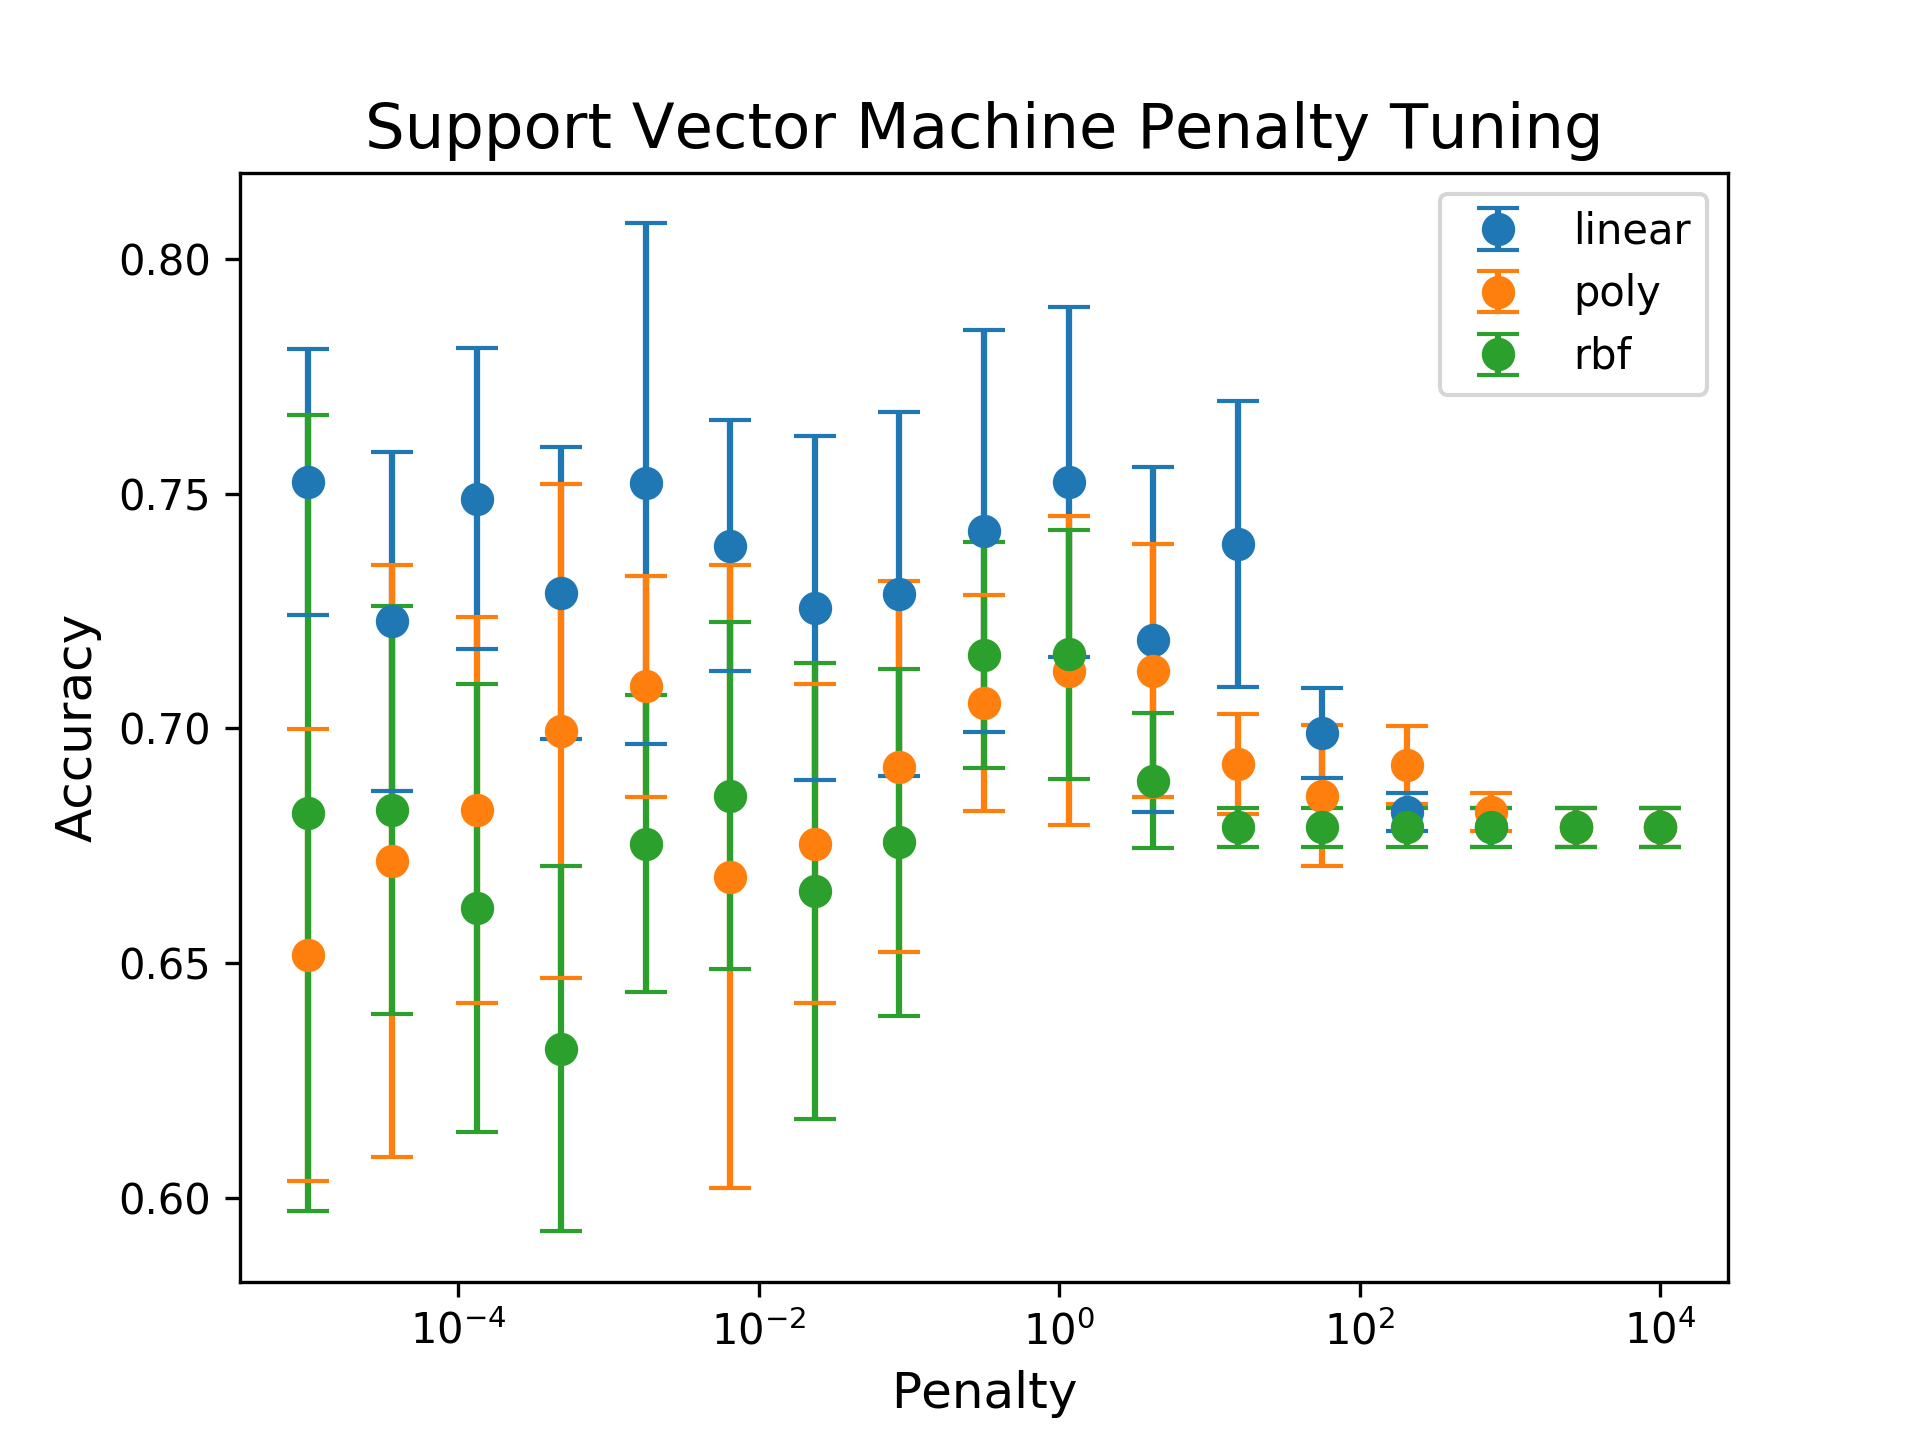
\includegraphics[width=0.42\textwidth]{../Figures/SVM_penalty_tuning.png}
	\caption{Cross validated accuracies for different penalties of the support vector machine.}
	\label{CV_SVM}
\end{figure}
\clearpage
\begin{figure}[h!]
	\centering
	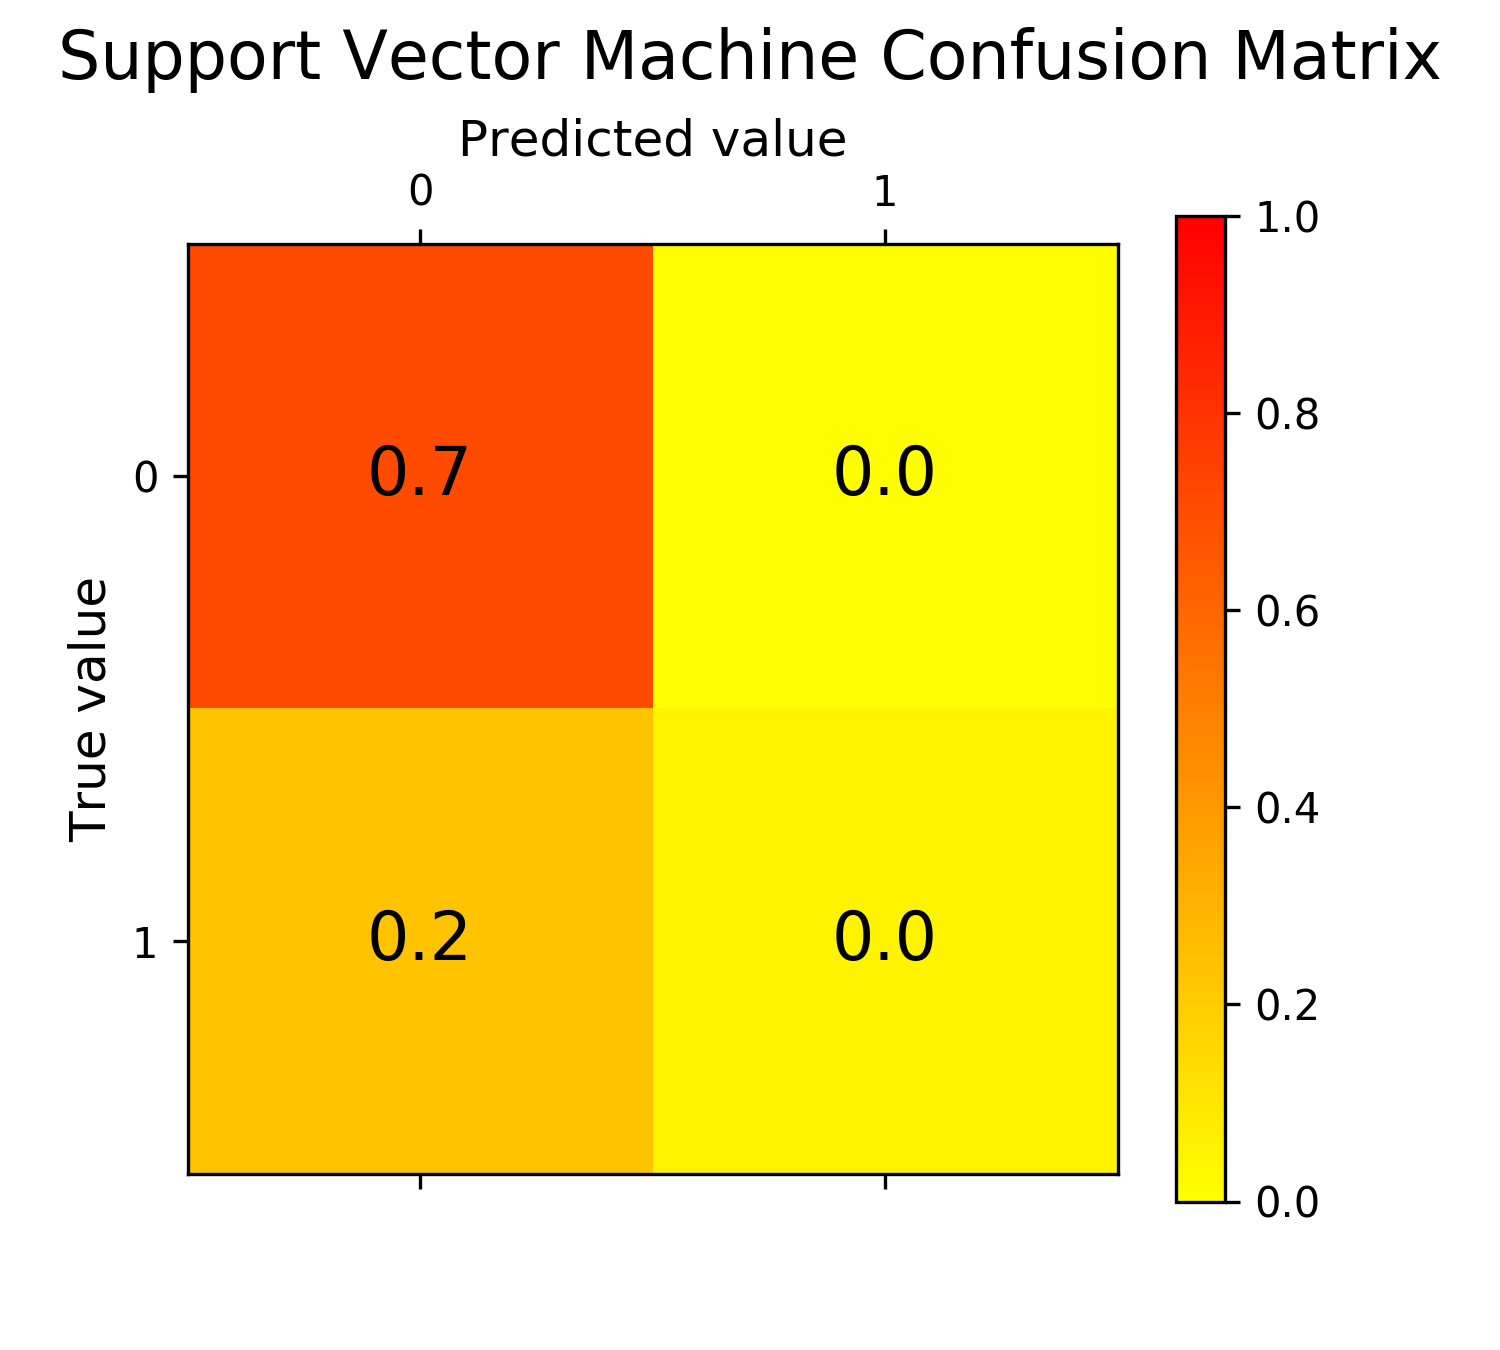
\includegraphics[width=0.45\textwidth]{../Figures/CM_SVM.png}
	\caption{Confusion matrix for best support vector machine model.}
	\label{CM_SVM}
\end{figure}

Figure \ref{CV_SVM} shows the 5-fold cross validated accuracies for different penalties for a support vector machine model using three different kernels. The linear kernel consistently performs better than the other kernels for all penalty choices. Therefore the linear kernel was chosen for performing feature selection. For the linear kernel there are, as for the logistic regression model, no significant improvements to be made by changing the penalty. However, we see that in this case also a large penalty limits the accuracy to just below 0.7. Figure \ref{CM_SVM} shows the confusion matrix of a support vector machine model using the linear kernel and the best penalty determined from figure \ref{CV_SVM}. Similarly to the other models, the support vector machine has the largest contribution to the accuracy from correct prediction of surviving patients, whilst most dead patients are labeled incorrectly.  The support vector machine achieves an accuracy of $0.752\pm0.050$ using the linear kernel and the corresponding optimal penalty $\lambda=1$. In contrast with logistic regression and random forest, the support vector machine required considerably more time to train.


\subsection{Feature selection}
Figure \ref{feature_imp_RFC} shows the feature importance measures from the random forest model. The measures show that there are some features of little importance and some features of high importance. The less important features are smoking, diabetes, anaemia, high blood pressure and sex, while the most important features are serum sodium, platelets, CPK, age, ejection fraction and serum creatinine. Notably, the most important features all have comparable importances (meaning that they are in the same order of magnitude).\\[2mm]
The results of the recursive feature elimination procedures for all the models are presented in figures \ref{elim_LR}, \ref{elim_RFC} and \ref{elim_SVM}. All three models agree that using 2-3 features can reproduce the results of the complete models, although they don't necessarily agree on the order of feature removal. Notably, the random forest model requires 3 features in order to reproduce the full model accuracy whilst the linear regression and support vector machine models only require 2. 
\begin{figure}[h!]
	\centering
	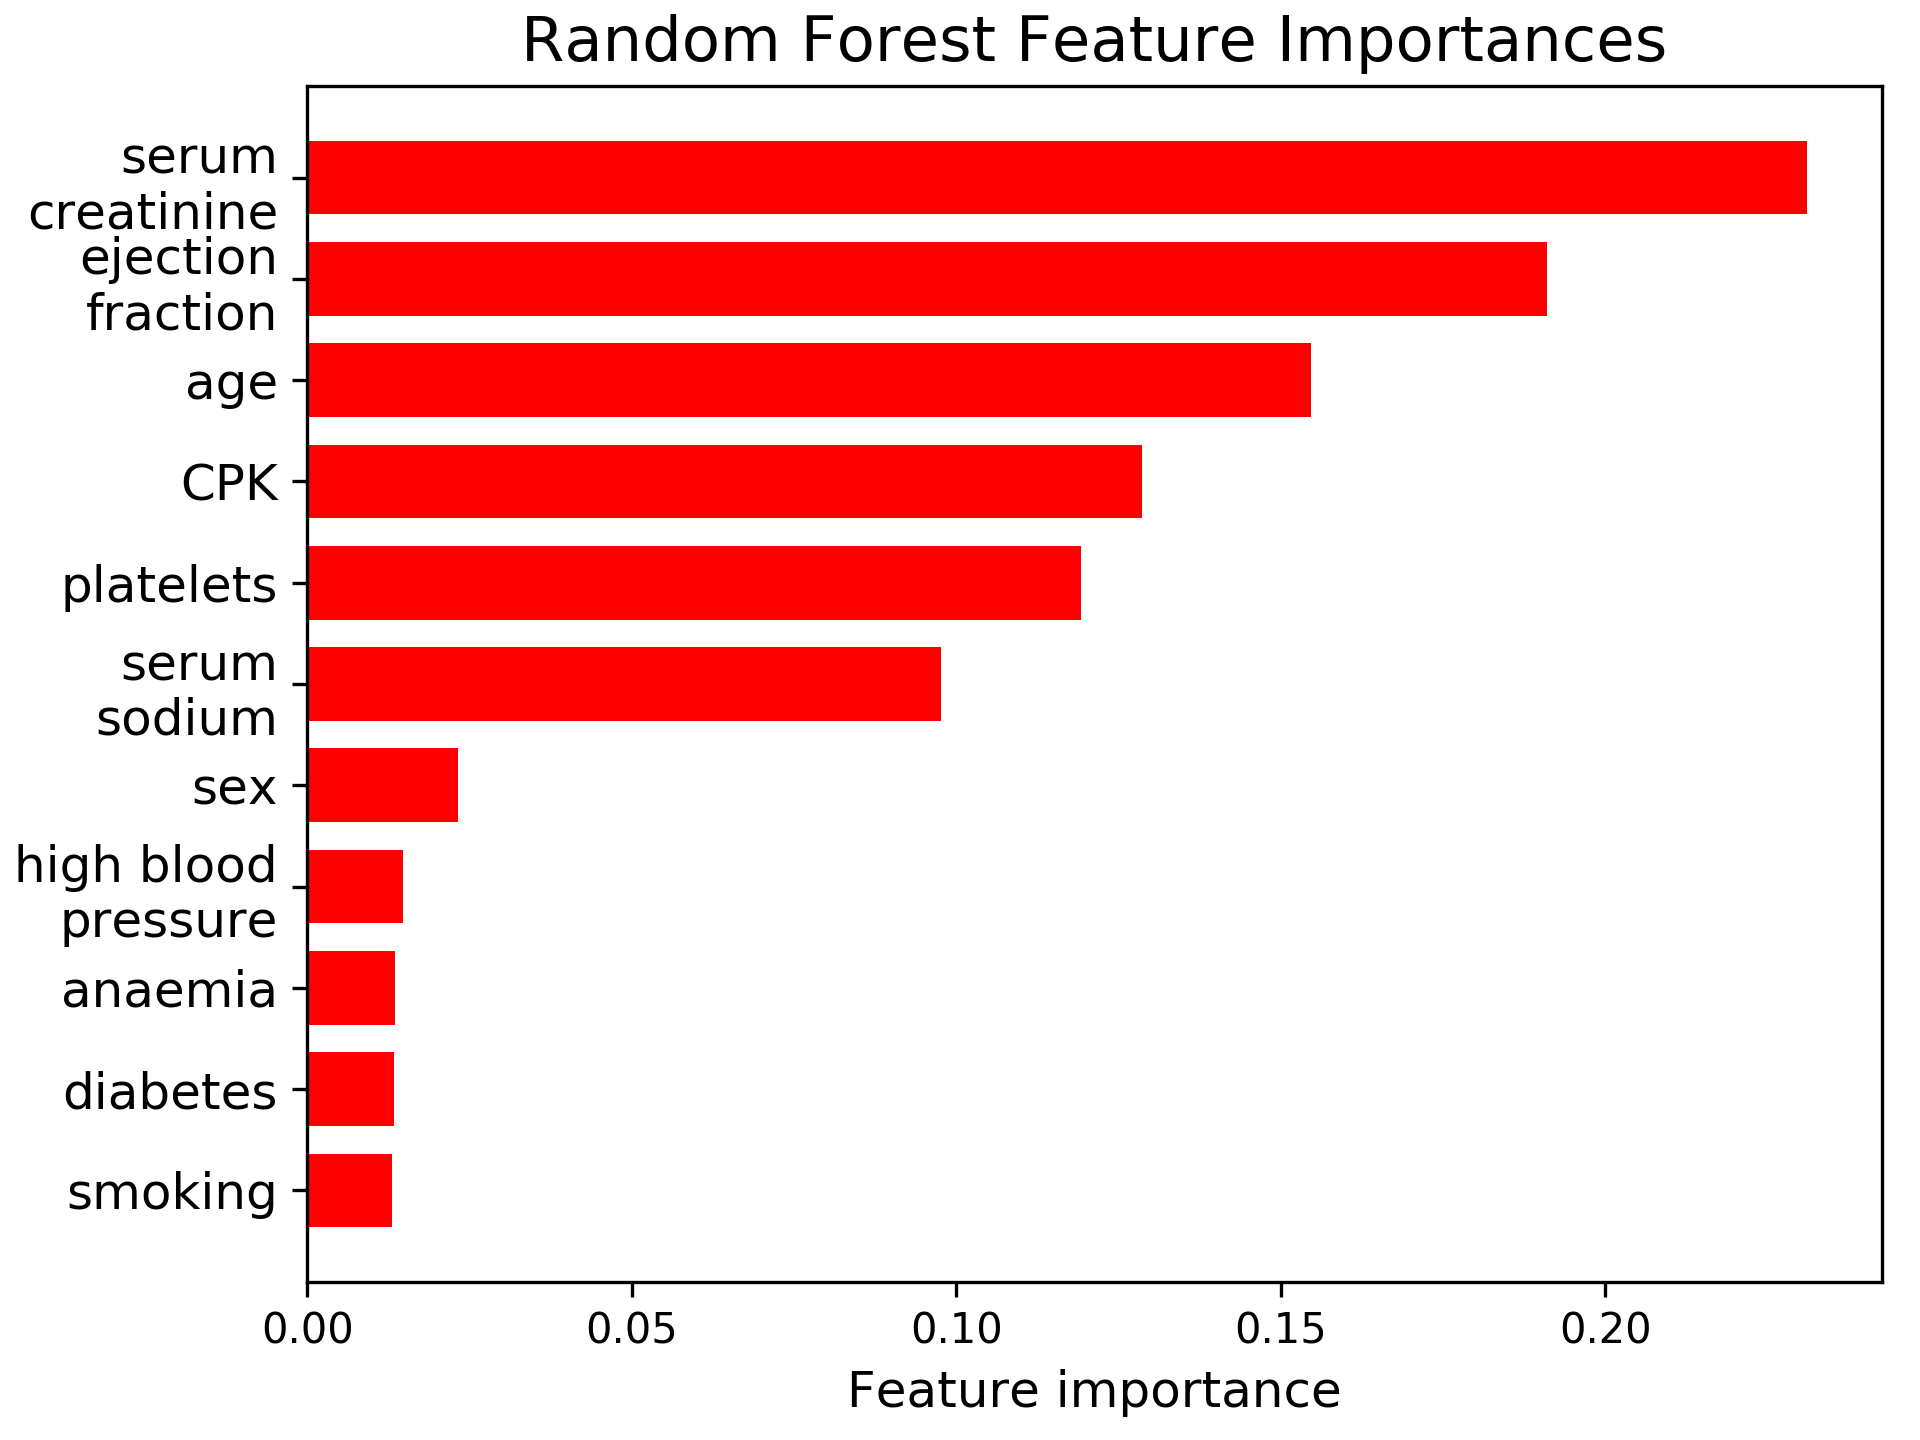
\includegraphics[width=0.42\textwidth]{../Figures/feature_importances_RFC.png}
	\caption{Feature importances in the random forest model. }
	\label{feature_imp_RFC}
\end{figure}

\begin{figure}[h!]
	\centering
	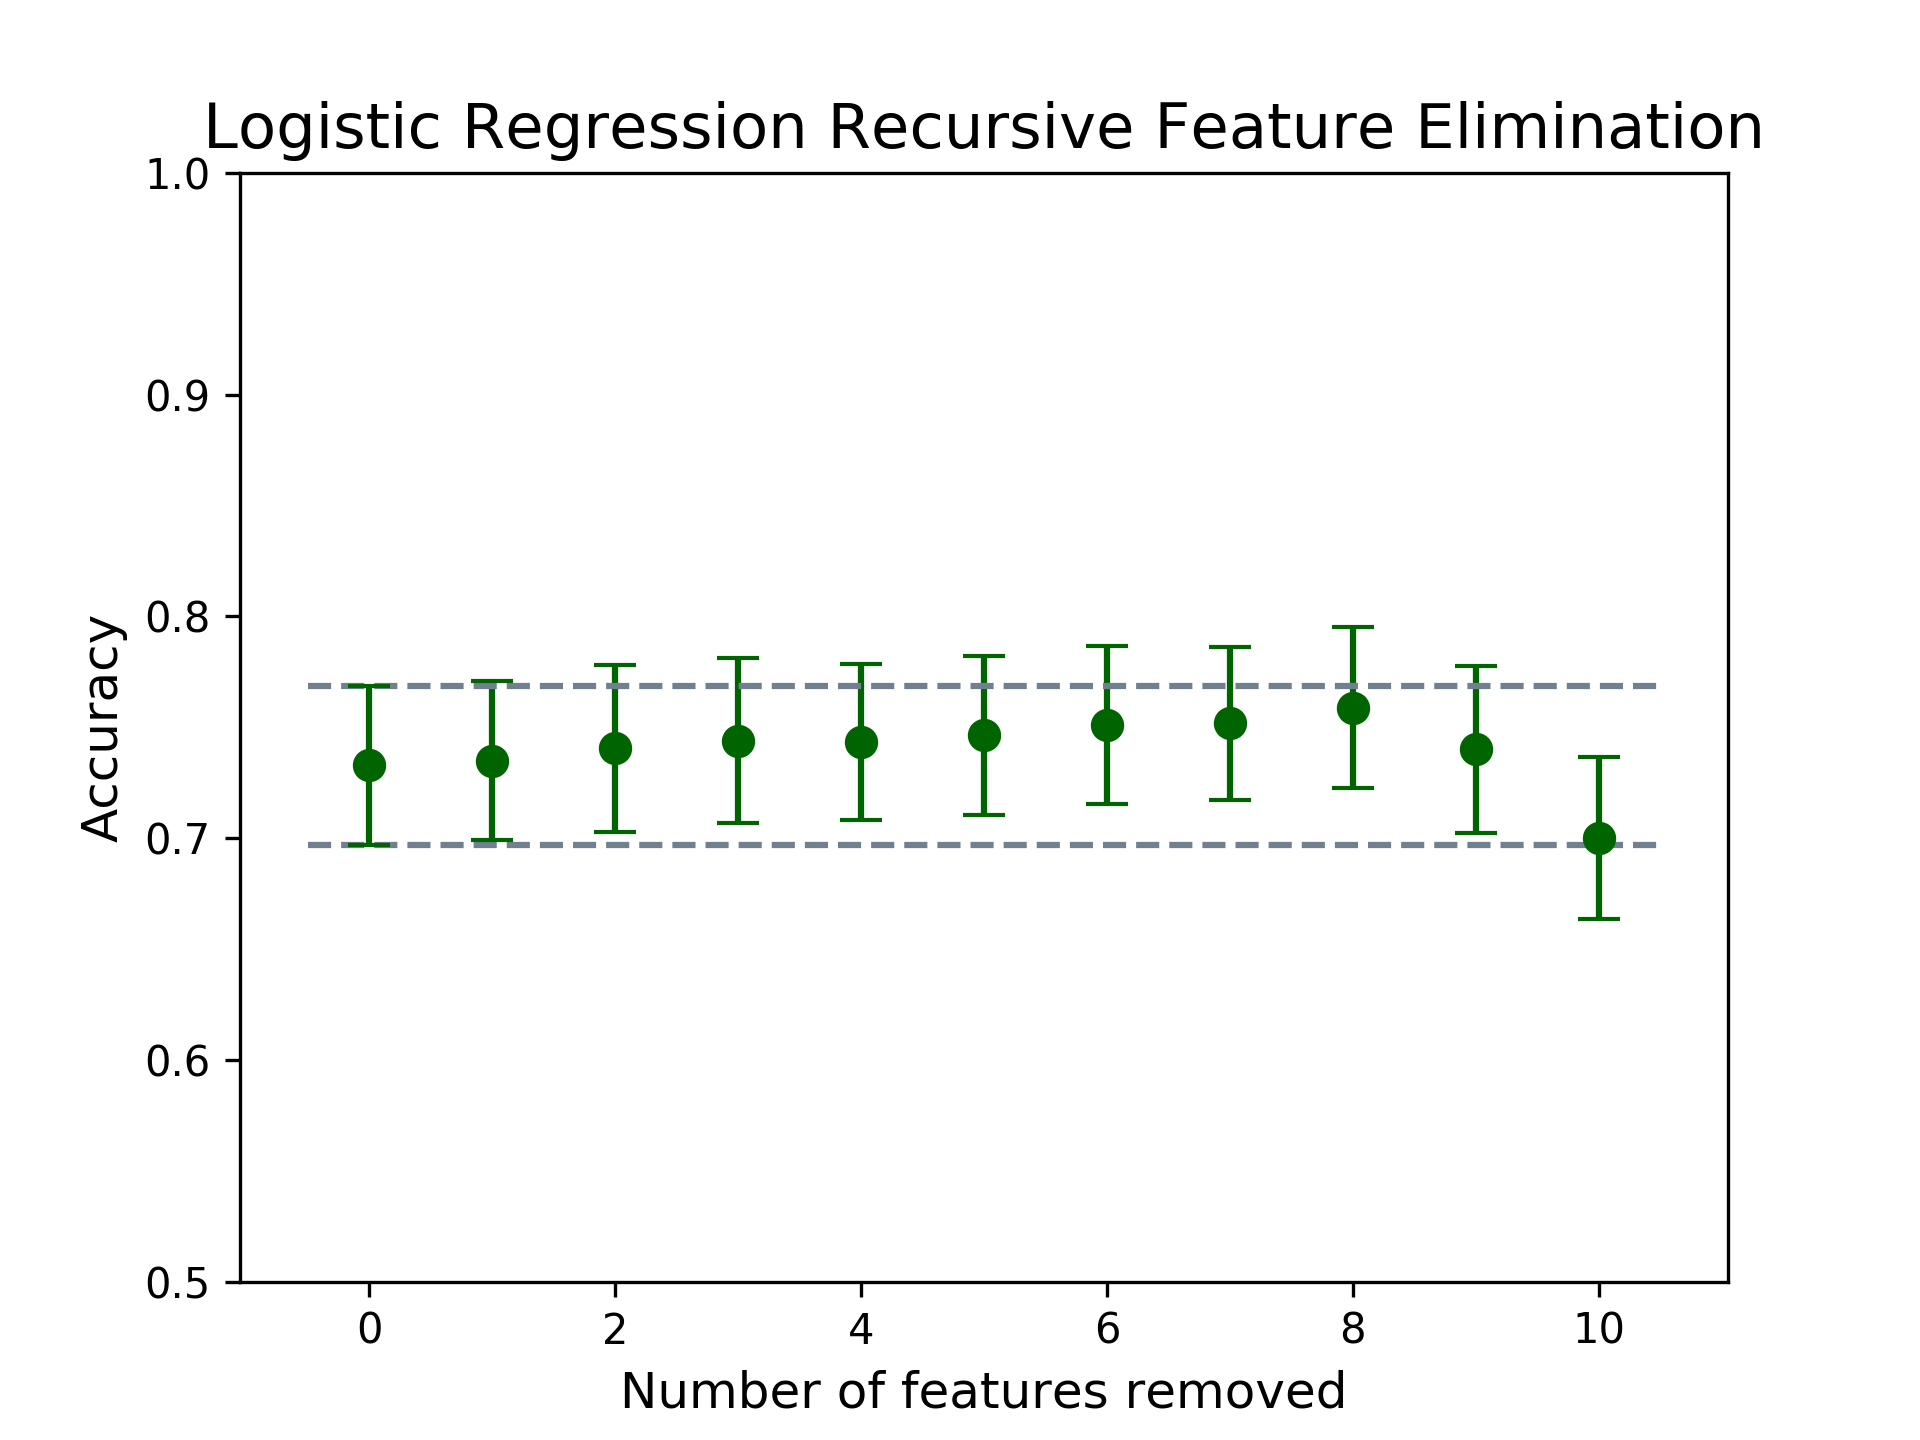
\includegraphics[width=0.42\textwidth]{../Figures/recursive_feature_elimination_LR.png}
	\caption{Results of recursive feature elimination for logistic regression. Order of removal: platelets, diabetes, serum sodium, creatinine phosphokinase, smoking, anaemia, sex, high blood pressure, age, ejection fraction and serum creatinine.}
	\label{elim_LR}
\end{figure}

\begin{figure}[h!]
	\centering
	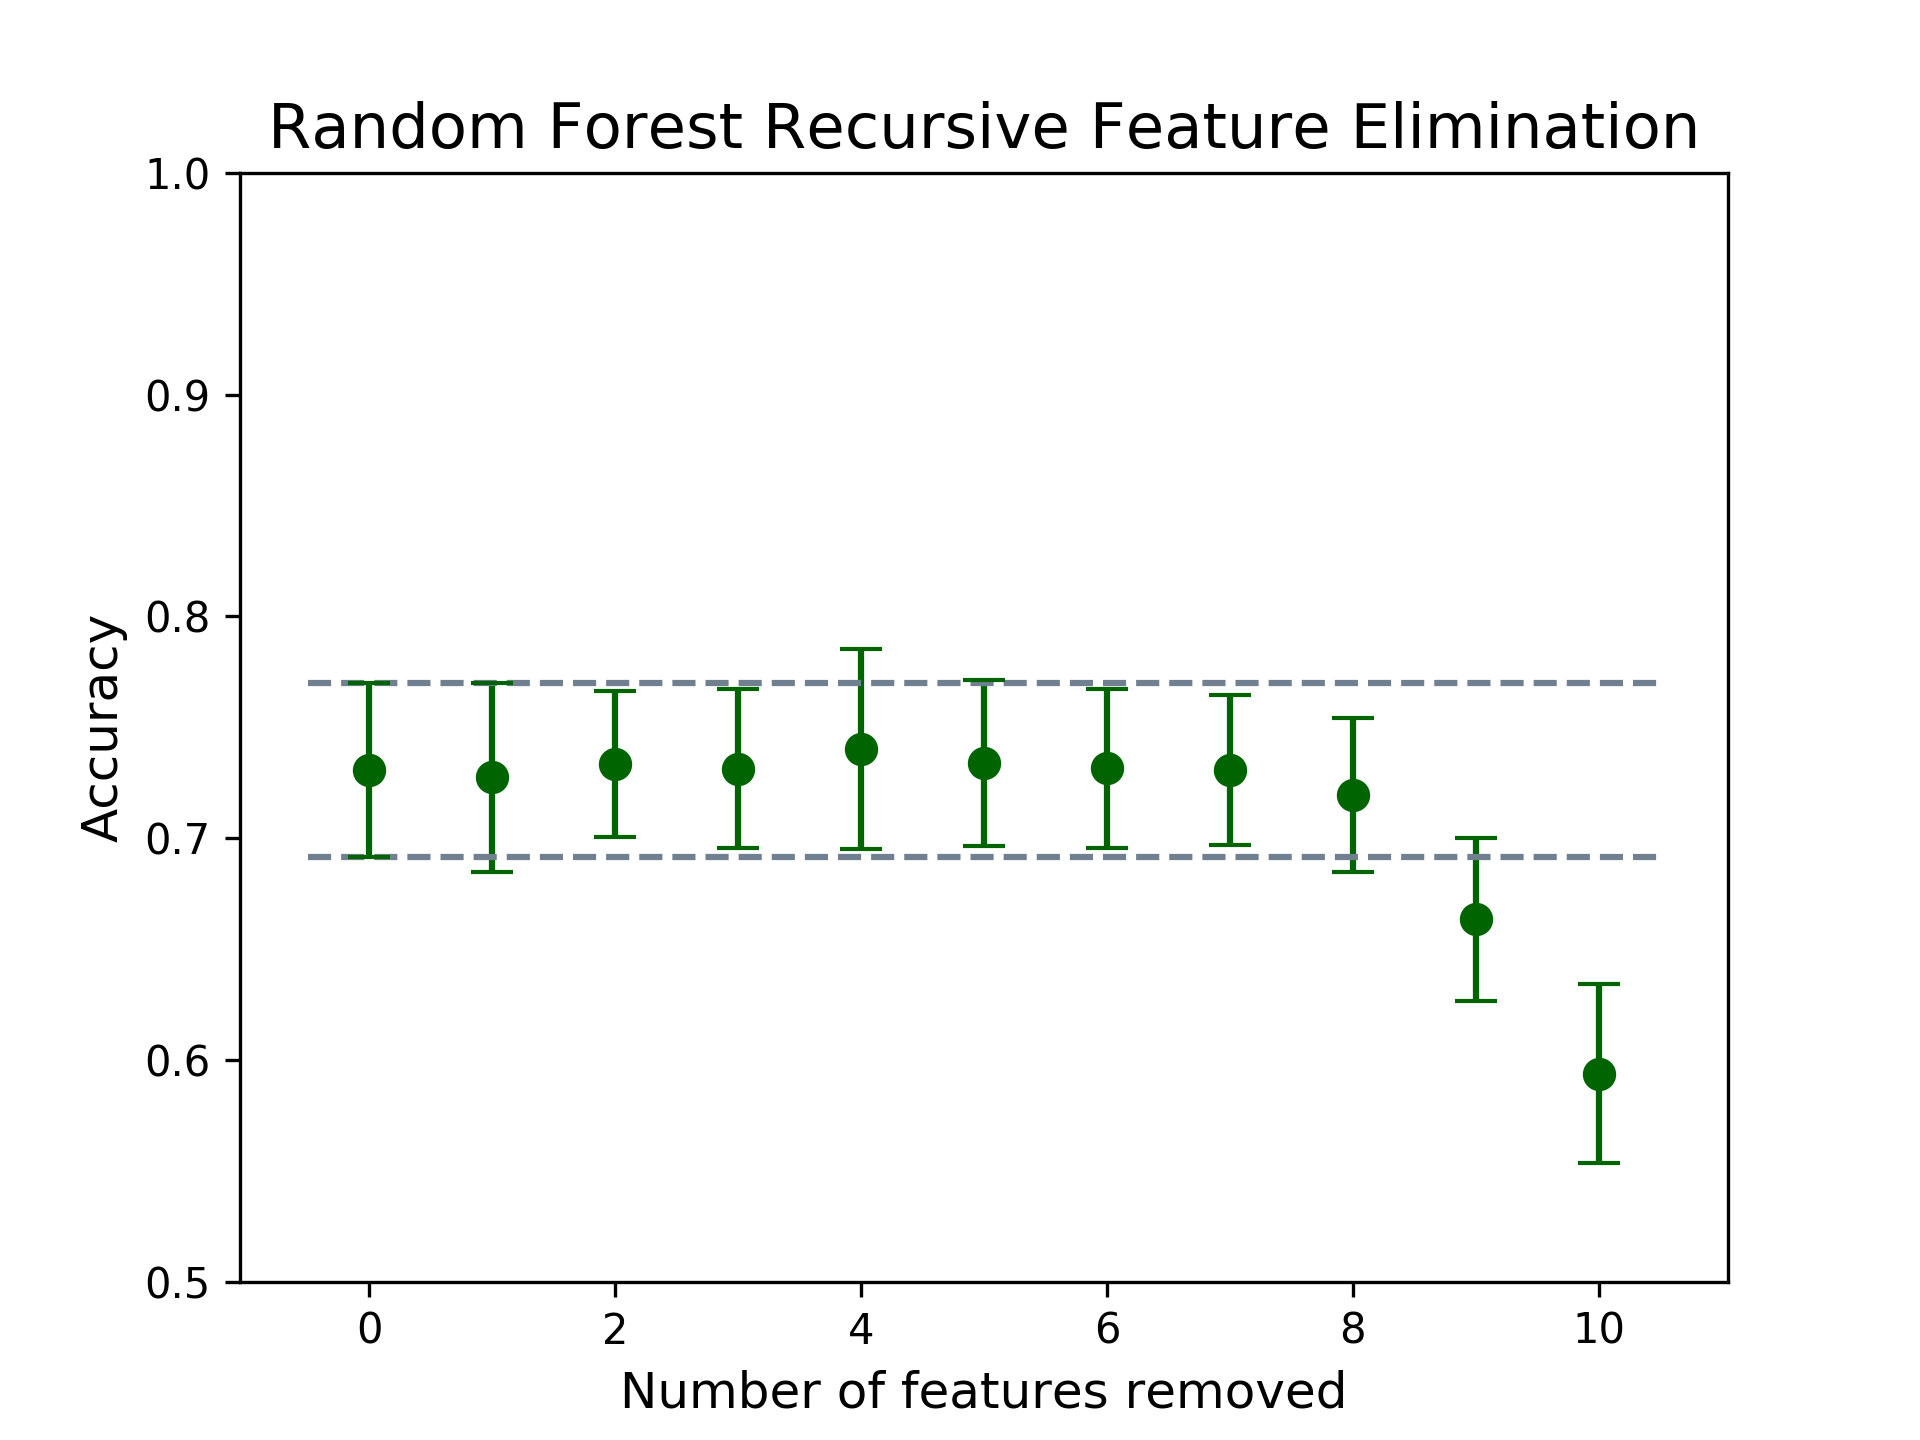
\includegraphics[width=0.42\textwidth]{../Figures/recursive_feature_elimination_RFC.png}
	\caption{Results of recursive feature elimination for random forests. Order of removal: smoking, diabetes, anaemia, sex, high blood pressure, serum sodium, creatinine phosphokinase, age, ejection fraction, serum creatinine and platelets.}
	\label{elim_RFC}
\end{figure}

\begin{figure}[h!]
	\centering
	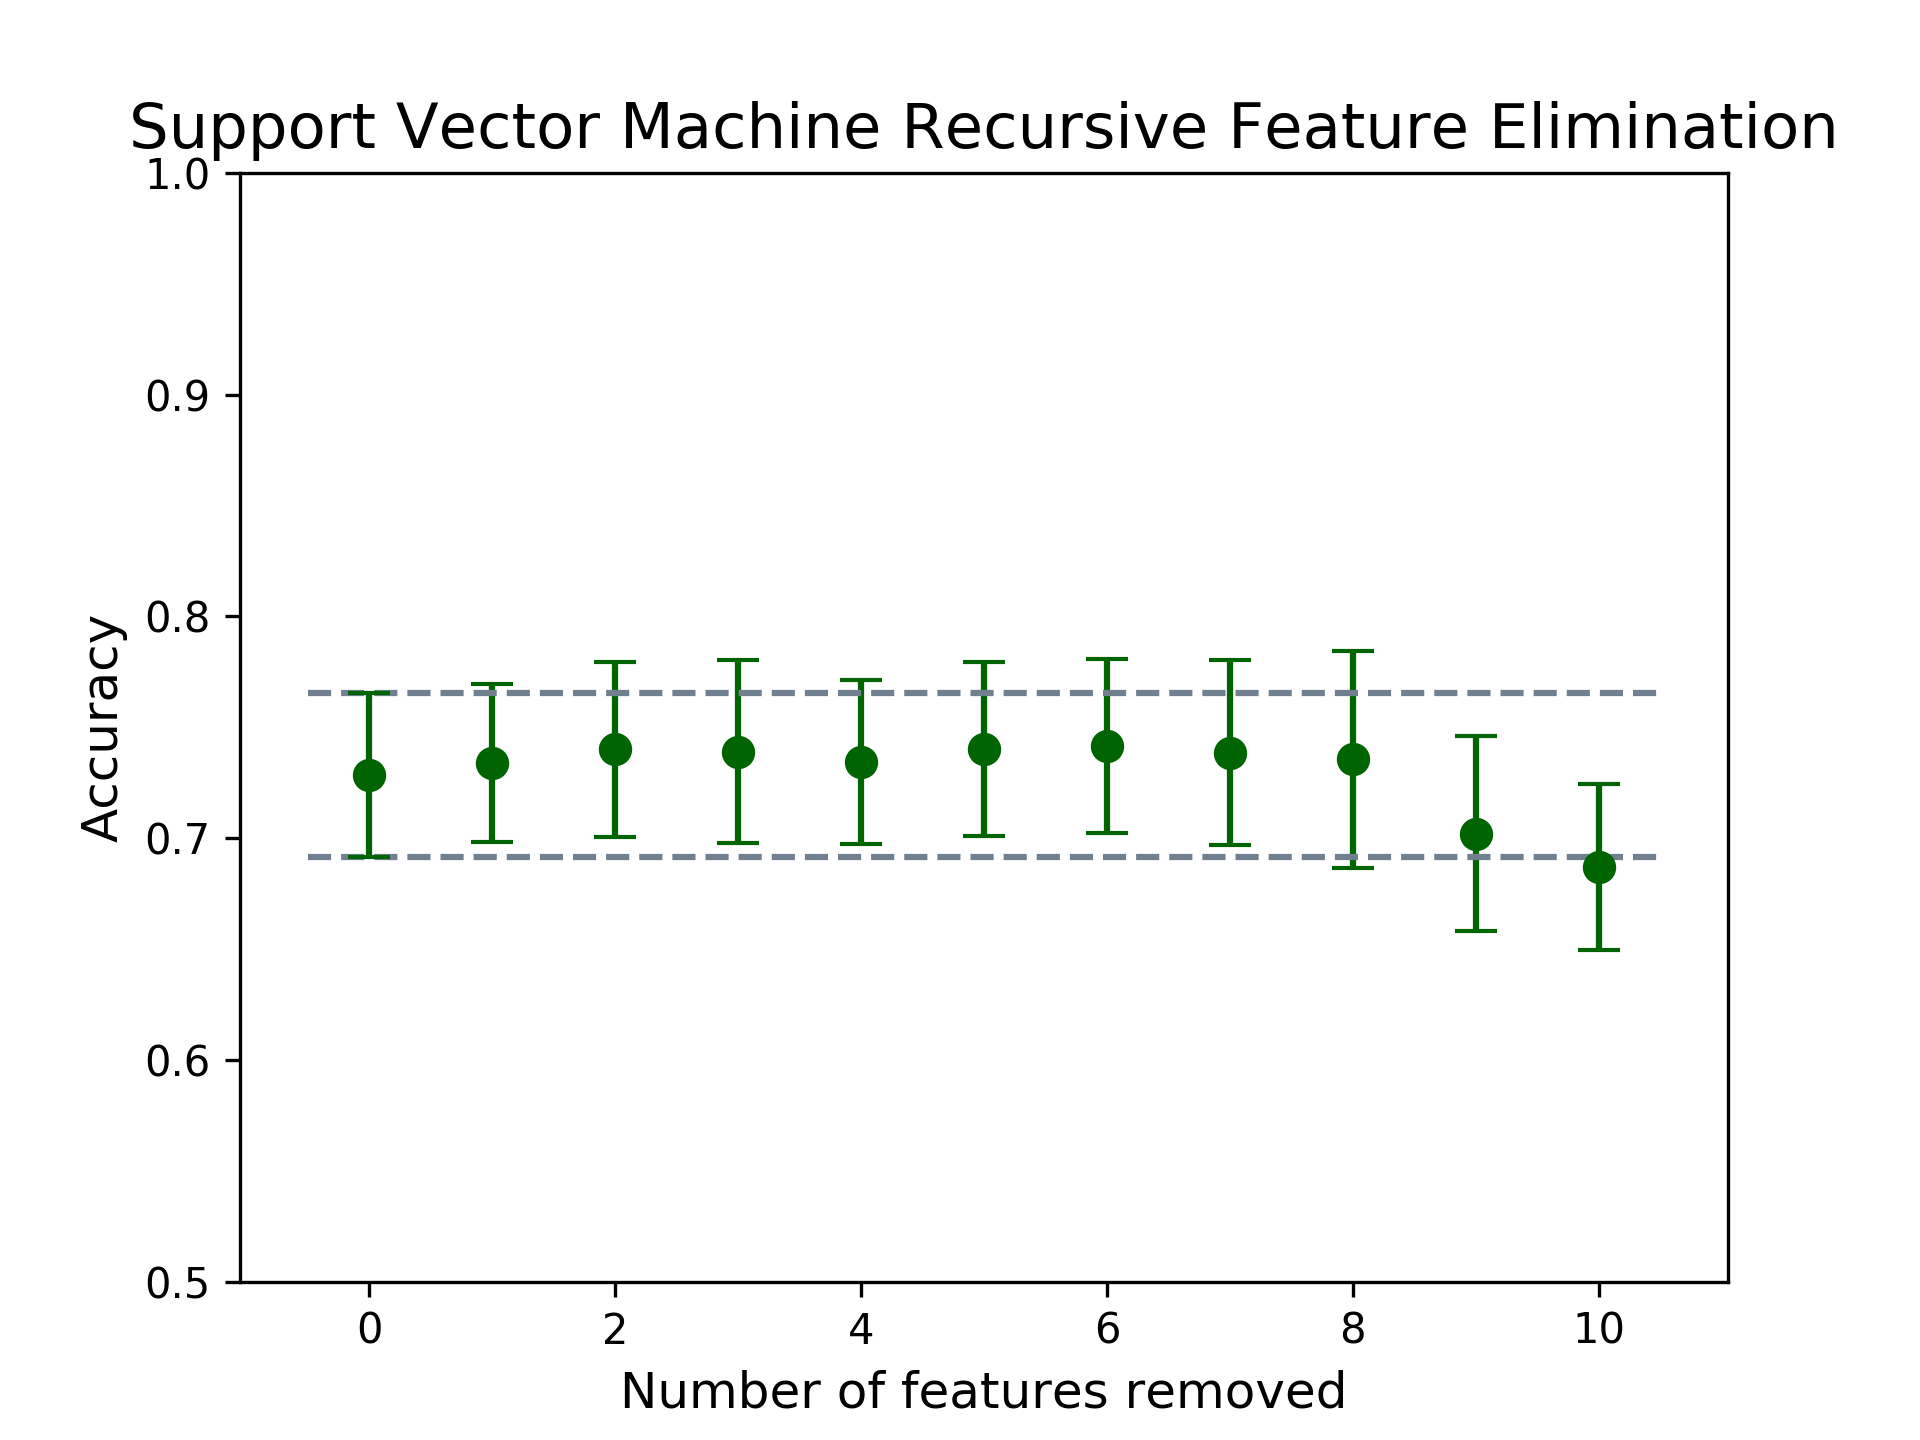
\includegraphics[width=0.42\textwidth]{../Figures/recursive_feature_elimination_SVM.png}
	\caption{Results of recursive feature elimination for support vector machines. Order of removal: platelets, diabetes, creatinine phosphokinase, anaemia, serum sodium, smoking, high blood pressure, sex, age, ejection fraction and serum creatinine.}
	\label{elim_SVM}
\end{figure}
\newpage
\section{Discussion}
For both the logistic regression model and the support vector machine, figures \ref{CV_LR} and \ref{CV_SVM} show that tuning the penalty parameter had little effect on the overall performance of the models. In both cases, the accuracy stabilises for higher penalties and varies for lower penalties, although the variation is much greater for the support vector machine. This is unexpected from the point of view of a bias-variance tradeoff analysis as one would expect there to be an optimal region for the penalty. Interestingly, the linear kernel outperformed the other kernels in the support vector machine. This is also unexpected, as it is less flexible than the other kernels. It is also worth mentioning that the time required to train a support vector machine was considerably higher than that of logistic regression and random forest.\\[2mm]
For random forests, figure \ref{CV_RFC} shows that increasing the number of trees beyond 50 led to no significant improvement in the model accuracy. This is lower than typical values which are of magnitude $10^2$. \cite{ESL} Interestingly, tuning the hyperparameters of the decision trees in the forest showed no clear patterns of improvement; figure \ref{hyperparam_RFC} shows that using the optimal choice of hyperparameters does not outperform the default parameters used in figure \ref{CV_RFC}. \\[2mm]
Overall, all the models achieved a similar accuracy ($\approx 0.75$). In addition, the confusion matrices (figures \ref{CM_LR}, \ref{CM_RFC} and \ref{CM_SVM}) show that the largest contribution to the accuracy came from correctly predicting surviving patients. Out of the dead patients, a greater fraction were predicted to survive in all the models. The models' failure to accurately predict patient deaths likely stems from the imbalance in the data set (out of the 299 patients, only 96 patients died). \\[2mm] 
There is an interesting difference between the feature importance measures of the random forest (figure \ref{feature_imp_RFC}) and the results of the recursive feature elimination procedures (figures \ref{elim_LR}, \ref{elim_RFC} and \ref{elim_SVM}). Judging by the feature importances, a larger amount of features should be important to the model compared to what we found using recursive feature elimination. Also, the importance measures fall off exponentially whereas the recursive feature elimination shows a discontinuous distinction between the important and the unimportant features. The main difference between the two methods is that the feature importance measures were determined based on all the features, whilst the recursive feature elimination considers a decreasing set of features. The discrepancy between the two results indicates that some of the features contain some of the same information without being correlated. For instance, high levels of serum sodium or serum creatinine both indicate kidney issues, which can increase the likelihood of mortality. However, the discrepancy may also be explained by how the random forest treats the data differently from logistic regression and support vector machines. Whereas random forests use hard cut-offs to make binary splits in the feature space, both logistic regression and support vector machines consider continuous transformations of the data. The results of this can be seen in the recursive feature elimination procedure for the random forest (figure \ref{elim_RFC}), which is unlike the other two in the sense that it requires a greater number of minimum features to achieve an accuracy similar to the complete model. \\[2mm]
In the recursive feature elimination, the order of removal for the logistic regression model and the support vector machine agree almost exactly (see figure \ref{elim_LR} and \ref{elim_SVM}). Importantly, the two methods agree on the three most important features: age, ejection fraction and serum creatinine. In addition, the models also agree that ejection fraction and serum creatinine are sufficient for reproducing the accuracy of the full models. It is reasonable for ejection fraction to be one of the most important features for this patient group, since they all suffer from left ventricular systolic dysfunction. In a sense, the ejection fraction is a measure of the severity of the patients heart failure. It is also reasonable for serum creatinine to be one of the most important features, since the serum creatinine levels are an indicator of kidney health. The random forest recursive feature elimination has ejection fraction, serum creatinine and platelets as the three most important features (see figure \ref{elim_RFC}). This is in contrast to logistic regression and the support vector machine which considered platelets to be the least important feature. However, this is another argument supporting the claim that the features share information other than a direct correlation. Moreover, the importance of platelets is noticeable in the feature importance measures of the random forest (figure \ref{feature_imp_RFC}), which explains how platelets was not removed during the early stages of the recursive feature elimination procedure. 


\section{Conclusion}
The aim of this project was to use supervised machine learning methods for identifying the most important features in the survival and death of heart failure patients in order to provide an indication of possible causes of death in this patient group. The features considered stem from medical records of 299 heart failure patients as collected by Ahmad et al. \cite{dataset_article} The project considered three supervised machine learning methods: logistic regression, random forests and support vector machines. Using the optimal hyperparameters for each model (as determined by 5fold cross validation), the models achieved an accuracy of $0.746\pm0.041$, $0.756\pm0.022$ and $0.752\pm0.050$, respectively. As these are all within the confidence intervals of each other, there is no reason to prefer a particular model. However, the support vector machine required considerably more time to train, thus from an efficiency point of view it is recommended not to use this method for similar data. Moreover, each model was most successful in predicting survival. Tuning the hyperparameters of the methods had little to no effect on the overall performance. For feature selection, recursive feature elimination was used. Each method found that 2-3 features were sufficient for reproducing the accuracy of the full model. All the models found ejection fraction and serum creatinine to be among the top three most important features. However, random forests placed significant importance on platelets, which logistic regression and the support vector machine considered to be the least important feature.  \\[2mm]
The models used in this project all had a similar performance and failed to classify the same group of patients. Future work is needed to understand the relationship between this patient group and the models. In particular, whether the models fail to classify the patients for the same reason, e.g. lack of information in the data or outlier effects. In addition, it could be of interest to investigate a larger and more balanced data set, potentially with more features. Since each model achieved similar results, there is reason to believe that another supervised machine learning method would not be able to achieve a higher accuracy.
\bibliographystyle{unsrtnat}
\bibliography{references.bib}

\end{document}